
\documentclass[12pt,english]{report}
\usepackage{WSU}
\usepackage[T1]{fontenc}
\usepackage{xcolor}
\usepackage{booktabs} % used for tables
\usepackage{multirow} % used for tables to merge multiple rows
\usepackage{bigdelim} % used for tables to set spacing
\usepackage{bigstrut} % used for tables to set spacing
\usepackage{graphicx} % used for includegraphics
%\usepackage{subfigure} % allows the use of subfigures

\usepackage{epstopdf}  %for eps
\usepackage{floatrow}
\usepackage{geometry,array,graphicx,float,caption}
%% front pages

\usepackage[framed,numbered,autolinebreaks,useliterate]{mcode} % used to insert code
\usepackage{geometry,array,graphicx,float,caption}
\usepackage{url}
\usepackage{rotating} % for sidewaystable
\usepackage{pdflscape} % for sideway figure
\usepackage{comment}
\usepackage{array,tabularx,float}

\usepackage[flushleft]{threeparttable} % add note to table
\usepackage{epstopdf}  %for eps

\usepackage{amsmath}
\usepackage{natbib}  % for citation
\usepackage{verbatim} 

\usepackage{hyperref}

\usepackage{caption}
%\usepackage{subcaption}
%\captionsetup{compatibility=false}

\usepackage{floatrow}
\newfloatcommand{capbtabbox}{table}[][\FBwidth]
\usepackage{blindtext}


\usepackage{verbatim} 
\usepackage{paralist} % for inline list

\setcitestyle{authoryear,open={(},close={)}}

\begin{comment}

\usepackage{hyperref}

%\usepackage{indentfirst}
% sub section 
%\setcounter{section}{-1}
%\usepackage{titlesec}  % set subsubsubsub section
\setcounter{secnumdepth}{5} % set subsubsubsub section
%\usepackage{listings} % insert code

%\titleformat{\paragraph}
%{\normalfont\normalsize\bfseries}{\theparagraph}{1em}{}
%\titlespacing*{\paragraph}{0pt}{3.25ex plus 1ex minus .2ex}{1.5ex plus .2ex}
\usepackage{array,tabularx,float}
\setlength\extrarowheight{2pt}
\usepackage[nottoc]{tocbibind} % This add reference page number to tableofcontents


\setcounter{tocdepth}{2}
%level -1: part, 0: chapter, 1: section, etc.
\end{comment}





\begin{document}
%-----------------------------------------------------------------------
%  Modified fields
%-----------------------------------------------------------------------%
%\begin{comment}

\newcommand{\authorfirst}{Shuai}
%\newcommand{\authorMI}{}
\newcommand{\authorlast}{Wang}
\newcommand{\degreefull}{Doctor of Philosophy}  % force hyphenation at syllables if line breaks are required
\newcommand{\degreeshort}{Ph.D in Engineering Program}
\newcommand{\dept}{Department of Biomedical, Industrial and Human Factors Engineering }
\newcommand{\institution}{Wright State University}
\newcommand{\thesisordissertationlc}{Models and Methodology for Optimal Financial Aid Allocation for a State University}%
%\newcommand{\thesistitle}{Models and Methodology for Optimal Financial Aid Allocation for a State University}
\newcommand{\bachdegreeshort}{B.S., Management} % Bachelor degree short
\newcommand{\bachinstitution}{Dalian Jiaotong University} % Bachelor degree institution
\newcommand{\bachyear}{2011}% Bachelor degree year
%No spaces should be before or after this title.
%\newcommand{\pdfsubject}{a short paraphrase of your title or focus of your thesis}
\newcommand{\pdfkeywords}{keyword 1, keyword 2, keyword 3, keyword 4}
\newcommand{\yearcomplete}{2016}
% set pdf file info
%\hypersetup{
%                     pdfauthor={\authorfull},
%                     pdftitle={\thesistitle},
%                     pdfsubject={\pdfsubject},
%                     pdfkeywords={\pdfkeywords},
%                     }

%\end{comment}
%-----------------------------------------------------------------------
%  Thesis Advisor, Department Chair, Dean of Graduate Studies
%-----------------------------------------------------------------------
\newcommand{\thesisdirector}{Xinhui Zhang}
\newcommand{\thesisdirectortitle}{Ph.D.}
\newcommand{\director}{Frank Ciarallo}
\newcommand{\directortitle}{Ph.D.}
\newcommand{\graddean}{Robert E. W. Fyffe}
\newcommand{\deantitle}{Ph.D.}
%-----------------------------------------------------------------------
%  Final Examination Committee
%-----------------------------------------------------------------------
\newcommand{\fecone}{Xinhui.Zhang, Ph.D.}
\newcommand{\fectwo}{Carolin Gao, Ph.D.}
\newcommand{\fecthree}{Pratik Parikh, Ph.D.}
\newcommand{\fecfour}{Nan Kong, Ph.D.}
\newcommand{\fecfive}{Subhashini Ganapathy, Ph.D.}
%=============================
%  Begin document!
%=============================
%
%Don't touch

\begin{comment}
\newpage
\thispagestyle{empty}
\normalem
\pagenumbering{roman}
\pagestyle{plain}
\setcounter{page}{0}
\rhead{\today}
\maketitle
\end{comment}
%\doublespace





%\newpage %shuai
%still don't touch.   
%=============================
%  approval sheet shuai
%\thispagestyle{empty}
%\renewcommand\baselinestretch{2}
%\begin{singlespace}
%\signaturepage
%\end{singlespace}
%\newpage  %shuai
%=============================


%
%=============================
%  Abstract
%=============================
\newpage
\setcounter{page}{3}
\vspace{2in}
%
\begin{singlespace}
\begin{center}
  ABSTRACT
\end{center}

\begin{comment}
\noindent{\small{\authorlast, \authorfirst},
		 {\degreeshort, \dept, \institution}, 
		 {\yearcomplete}, 
		 {\thesisordissertationlc}}

\end{comment}

\end{singlespace}
\vspace*{.5in}	
%\pdfbookmark[0]{Abstract}{Abstract}
%\phantomsection
%The abstract should succinctly summarize the contents of the thesis, stating the problem, the procedure or methods used, the results, and any conclusions.  Doctoral dissertation abstracts should not exceed 350 words.
Financial aid design, allocation, and optimization is an important part of enrollment management and could have a profound impact on the financial health of a higher institution. For many universities, tuition takes a significant portion of their income; excess use of financial aid could reduce tuition income, yet insufficient use of financial aid would reduce enrollment quality and undermine tuition income; the optimal allocation of financial aid is non-trivial and has been a challenge for the enrollment office at many universities.

This research proposes a set of models and methodology to solve the optimal allocation of financial aid awards to students. The methodology is composed of two parts. The first part is to predict the response to financial aid from students with various socioeconomic backgrounds; the second is the allocation of financial aid among these students to maximize revenue. 
The first phase is the development of predictive models to derive the response, in terms of probability of acceptance of financial aid, from students with various socioeconomic characteristics. 
This is accomplished through the investigation and development of logistic regression models which predicts 1) the probability of enrollment of an applicant, and 2) the probability of graduation and the number of years of study of each applicant, given that he/she enrolls. The second phase is a mathematical model designed to allocate financial aid to applicants with an objective to maximize the revenue, which is composed of tuition minus scholarship allocated over the years, plus the state share of instruction (SSI) once the student graduates. These results are then post-processed to obtain managerial insights and to derive policies. 

The models have been adopted by a state university in Ohio and results suggested noticeable financial benefits. The solution of the financial aid allocation problems will contribute significantly to research studies in enrollment management.


\newpage 


\begin{comment}
%=============================
%  List of symbols (Optional)
%=============================
\newpage
%\renewcommand\baselinestretch{1.5}
\begin{singlespace}\begin{center}
  \textbf{\Huge{List of Symbols}}
\end{center}

%%%%%
\begin{flushleft}{\large Chapter 3} \end{flushleft}
\begin{tabular}{p{0.75in}l}
   $h$ & {Plate thickness}\\
   $L$ & {Plate length}\\
\end{tabular}
\end{singlespace}
	
\end{comment}

%=============================
%  Table of contents, etc.
%=============================
%\renewcommand\baselinestretch{1.5}
%\begin{singlespace}
%\tableofcontents
%\newpage %shuai

%\listoffigures
%\newpage %shuai

%\listoftables 
%\newpage %shuai

%\end{singlespace}



\begin{comment}

%=============================
%  Acknowledgments
%=============================
\newpage
\thispagestyle{plain}
\setlength{\parindent}{0em}
\begin{center}
{\huge Acknowledgment}
\end{center}

I would like to take this opportunity to extend my thanks to\ldots If you have multiple paragraphs, the first should not be indented to match the style of the rest of the thesis

\setlength{\parindent}{2em}
Any additional paragraphs should be indented as such.  Remember to thank your advisor and committee members.
%
%=============================
%  Dedication
%=============================
\newpage
\thispagestyle{plain}
\vspace*{3in}
\begin{center}
Dedicated to\\
Somebody Special (Wife or husband works well here)
\end{center}	
\end{comment}

%=============================
%  Begin Chapters
%=============================
\newpage
\setcounter{page}{1}
\pagenumbering{arabic}

\chapter{1    Introduction to College Enrollment and Financial Aid Allocation}
%\section[Introduction]{}

\section{Enrollment Management and Financial Aid}
%~\citet{enrollment_ref1} was the first book published about the enrollment management. In the book, the authors proposed that it is beyond an organizational concept in that it is both a process and a series of activities that involve the entire campus. The lifetime of enrollment management begins from the student's initial contact with the institute and ends at the graduation. As an activity, enrollment management is utilized to attract and retain students.

Enrollment management was coined by Dr. Jack Maguire \citep{maguire1976organized} and is used frequently to describe strategies and tactics to shape the enrollment of a higher learning institution to meet established goals \citep{kemerer1982strategies}.
Enrollment management is a series of processes and activities that follows a student's initial contact with the institute, transition to college, attrition, retention, and finally graduation \citep{hossler1990strategic}.
%As an activity, enrollment management is utilized to attract and retain students ~\citet{enrollment_ref1}. an organizational concept and a systematic set of activities designed to enable educational institutions to exert more influence on their enrollments \citet{enrollment_def2}. 

%For most universities in USA, the mission of enrollment~\citet{mission1,mission2,mission3} is to come up with strategies to increase the number of new students, to lead efforts to diversify the student body and to retain more students, and to help the university to enroll more high-ability students or students with special talents.

%In short, enrollment management is to approach, enroll and retain students that a college wants. As a process,~\citet{huddlestonenrollment2000} concluded that enrollment management is a research-based process that creates a synergy among recruitment, pricing and financial aid, academic affairs, student life, and constituent relations.

Enrollment management is critical to many colleges and universities \citep{braunstein1999measuring,maltzdecision,aksenovaenrollment} and has provided a fertile ground for advanced analytical studies. These studies can be categorized into the following areas: prediction of headcount \citep{aksenovaenrollment,changapplying2006}, financial aid allocation \citep{leedsthe2014,jacksonfinancial,dynarski1999does}, marketing strategies \citep{pandeyAdvertise}, retention studies \citep{grossinstitutional2015,dynarski1999does}, and course offering and evaluation \citep{SurjeetClassEnroll,luan2006courseoffer}. Data mining models and techniques, such as regression analyses, support vector machines, decision trees, neural networks etc., have been widely adopted in enrollment management studies. For details on some of these studies, please see \citep{luan2006data}.

%move this section when you describe financial aid in detail in later chapters.
%This research focuses on optimal allocation of financial aid. the Besides some special designed scholarships like sports scholarship, Valedictorian/Salutatorian scholarship,  the two most common scholarships that colleges provide are need-based and merit-based aid \citet{finacial_history}.   Need-based aid is designed to aid students regardless of academic ability and given exclusively based on need. The factors considered in this  scholarship includes student's family income, Free Application for Federal Student Aid (FAFSA).  Merit-base aid, on the other hand, only considering the academic performance such as ACT/SAT, GPA and school percentile. In practice, the aid converted to reduction of tuition, and fees like dorm payment, textbook, etc.

%When college starts to open the admission every year, the admission office will have a budget. So how to allocate the budget so that to attract as many student as the administrators they want, as well as maintain the quality, diversity, etc, becomes a issue to enrollment officers. The study on financial aid allocation is mainly focus on seeing how different scholarship policies exert impact the enrollment 

This research focuses on the optimal allocation of merit-based financial aid awards (or scholarships) to students in an effort to increase student enrollment. The use of financial aid has long been recognized as a tool for a university to attract high-talent students. For example, early studies \citep{heller1997student,jacksonfinancial,leslie1988economic} have shown that ``receiving a financial aid award has a significant positive effect on the likelihood that a student will enter the institution that has  made the financial aid offer'' and ``the effect of just receiving an award, regardless of the amount, equals or exceeds the effects of the amount of the award.''

Though financial aid design and allocation is an important part of enrollment management strategies, studies of financial aid are mostly limited to descriptive analyses such as causal effects of financial aid.  For example, \citet{hossler1989understanding} have consistently found that ``African American students and Latino students are more cost sensitive and more responsive to financial aid offers than majority students of similar socioeconomic background.''  \citet{braunstein1999measuring} found that for every every \$1,000 increase in financial aid, the probability  of  enrollment increased between 1.1\% and 2.5\%.  These studies, nevertheless, have not addressed the fundamental question to be answered: how to allocate limited financial aid awards to students with various socioeconomic backgrounds to reach institution goals such as to maximize its revenue. This is referred to as the optimal financial aid allocation problem.

\section{The Dilemma at An Exemplary University}
The solution to the optimal financial aid allocation, though could have a profound impact on the economic health of an institution, is non-trivial. For many universities, tuition is a significant portion of their income; excess use of financial aid  could reduce tuition income, yet insufficient use of financial aid would reduce enrollment and undermine tuition income; the optimal allocation of financial aid has created a challenging problem for the enrollment management teams at many universities -- Wright State University is such an example.   

Wright State University is one of the thirteen state universities within Ohio and had an enrollment of 17,779  in the 2013-2014 academic year. The university aims to provide affordable service with high quality education and is eager to grow its enrollment and revenue in the coming years.  The desire to grow, however, is faced with tough challenges because the university is competing with other flagship universities for high-talented students and with community colleges for students seeking affordability.  

Typically, growing competition for college students has resulted in greater amounts of university funds being invested in scholarships designed to influence the enrollment decisions of students. For private universities, a widely adopted approach is some variant of the ``Robin Hood'' strategy \citep{hossler2000role}, which raises tuition and uses large portions of the increase to provide financial aid to prospective  students in order to induce them to matriculate. 

This, however, is not an option for a state institution such as Wright State University. To provide affordable education, the state government has capped statewide tuition increases, and at the time of this writing has mandated the increase of tuition to be zero for the 2015 - 2016 year. More than 95\% of the students, whose tuitions contribute to 46.75\% of the university's revenue, come from the surrounding southwest Ohio region where the population remains steady with no dramatic increase in high school graduates. The effective use of institutional resources such as financial aid to increase enrollment has thus been the focus of university executives. 
 
%Though several questions have been raised, these questions boil down to what students should be awarded in scholarships and how much the scholarships should be, so as to maximize the total revenue for the institution, subject to various requirements such as the total availability of financial aid and the capacity of programs. 
%========================================
\section{Model and Solution Approach}
%========================================
To solve the optimal allocation of financial aid, it is necessary to solve two problems.The first one is to study the response to financial aid award or scholarship from students with various socioeconomic backgrounds; the second is the allocation of financial aid among these students to maximize revenue. In this study, the solution to the problem is composed of three phases as follows:  

\begin{itemize}
\item [(a)] The first phase is the development of predictive models to predict the sensitivity to financial aid from students with various socioeconomic characteristics. This is accomplished through logistic regression based models which predict 1) the probability of enrollment of an applicant, and 2) the probability of graduation and the number of years of study of each applicant, given that he/she enrolls. 

\item [(b)] The second phase is a mathematical model designed to allocate financial aid to applicants with an objective to maximize the revenue, which is composed of tuition minus scholarship allocated over the years, plus the state share of instruction (SSI) once the student graduates.

\item [(c)] The third phase is a policy analysis that translates the optimization results, in the form of the  amount of scholarship awarded for each student, into managerial insights and policy for implementation. 
\end{itemize}

As can be seen, the solution approach elegantly combines data mining (phases (a) and (c)) and optimization techniques (phase (b)). The successful solution of these problems will contribute significantly to research studies in financial aid allocation and bring noticeable financial benefits to many universities. 

The remainder of the report is organized as follows. Section 2 presents a review of related literature. Section 3 presents a predictive models based on logistic regression and Section 4 presents the mathematical models and techniques for computational improvement. Section 5 presents the policy development, implementation results, and future research. 


\chapter{2 Literature Review}
The literature review is composed of two parts; the first part is predictive models in enrollment management and the second part is optimization models for the allocation of limited financial aid in enrollment management.  

\section{Binary Prediction or Classification }

The problem to predict ``enroll'' or ``not enroll'' belongs to a set of problems with binary outcomes.  Typical tools used in binary prediction or classification include logistic regression, neural networks, and decision tree analysis \citep{han2011data}.

\section{Logistic Regression Technique}

Logistic regression, or binary logistic regression, is a member of the generalized linear model used to deal with problems in which the outcome or the dependent variable is binary (the independent variables, however,  can be either categorical or continuous). It is used, for instance, in predicting a) whether a patient has a certain disease based on the characteristics of the patient such as age, gender, weight, BMI, income, education, et al.; and b) whether a flight will be delayed based on weather, time of day, destination and origination, and the flight carrier et al. Logistic regression was successfully used in various marketing research studies; for details on some of these studies, please see \citep{logistic_application1,logistic_application2,logistic_application3,logistic_application4,logistic_application5,logistic_application6,logistic_application7,logistic_application8,logistic_application9,logistic_application10,logistic_application11,logistic_application12,logistic_application13}. 

\subsubsection{Logistics Regression Applications in Enrollment Management}
Logistic regression has been used mostly for predicting enrollment levels and models the probability of enrollment as a linear function of a set of predictor variables \citep{lr_summary}. The predictor variables in most research studies can be classified into two categories \citep{braunstein1999measuring}: (1) academic and demographic information, such as ACT/SAT scores, high school GPA, location, gender, ethnicity, first language, parents' education level, etc; and (2) economic related status like family income, tuition, financial aid, and scholarship. Though some research studies examined variables such as health and psychosocial condition, not all of these variables are readily available to all universities. 

\citet{lr_1_chang} presented a case study of data mining in enrollment management and used logistic regression to predict the probability that a student will be admitted. This probability is then used by the institution to form a referral pool of highly prospective students for direct marketing outreach. \citet{lr_2} chose logistic regression to predict two stages in admission and enrollment. In the first stage, they predicted the probability of acceptance of each applicant. The results helped institutes to understand the features of potential incoming students such as geographical diversity, ethnicities, and academic performance. In the second stage, the enrollment probability of an admitted student was calculated. In this stage, they found that academically strong students are less likely to enroll.

\citet{braunstein1999measuring} analyzed the impact of  financial and socioeconomic factors on enrollment. They found that, by using logistic regression, for every \$1,000 increase in the amount of aid offered, the probability of enrollment increased between 1.1\% and 2.5\%.

\citet{lr_aid2} applied logistic regression to see the impact of financial aid amounts on different racial groups. Their results shown that overall, grants and combinations of loans and grants have a positive impact on enrollment (having loans alone does not have a significant impact); however, different impact patterns were found among individual racial groups.

\citet{lr_retention2} used logistic regression to delve into the relationship between freshmen year retention and exposure to part-time faculty. Results show that as exposure to part-time faculty instruction increases, the odds of being retained decrease.

\citet{lr_alumni1,lr_alumni2} used logistic regression to predict if an alumnus will donate or not, and some of the best prospects of alumni association membership were found. 

%\paragraph{Logistic Regression Assumption}
%Logistic regression assumes \citet{lr_assumption1, lr_assumption2}: (1) independence: observations are independent from each other; (2) linearity: linear regression assumes that the outcome variable has a linear relationship with the independent variables, or in the case of logistic regression, a linear relationship between the logit of the independent variables and outcome variables; (3) normal distribution is not necessary or assumed for the dependent variable.

\begin{comment}

\paragraph{Goodness of Fit for Logistic Regression Model}
%There are many tests that can be applied to evaluate the effectiveness of a logistic regression model. Of them, four of the commonly used tests are (a) tests of individual predictors, (b) overall model evaluation, (c) validation of predicted probabilities, (d) goodness of fit statistics. \citet{lr_summary} 

Goodness of fit statistics are the most used in the evaluation of logistic regression model \citet{lr_summary} and several methods have been proposed. 

The most straightforward method of evaluation  is to calculate the accuracy of the fitted value.  A cut-of value (in percentage) , say 60\%, is chosen and any predicted value greater than the cut-off will be a successful prediction and any value below will be a failure. This analysis can be entered into a two-by-two table, called a 'classification table' (or 'confusion matrix') as shown below:  
  
   % Please add the following required packages to your document preamble:
% \usepackage{multirow}
\begin{table}[h]
\centering
\label{my-label}
\begin{tabular}{|c|c|c|c|}
\hline
     & \multicolumn{3}{c|}{Actual Class}       \\ \hline
\multirow{3}{*}{\begin{tabular}[c]{@{}c@{}}Predicted\\  Class\end{tabular}} &   & Yes   & No    \\ \cline{2-4} 
 & Yes & True Positive       & False Positive \\ \cline{2-4} 
& No  & \multicolumn{1}{l|}{False Negative} & True Negative  \\ \hline
\end{tabular}
\caption{Classification Table}
\end{table}

%The limitation of this measurement is that it does not have any measure of significance.This means that 99\% accuracy can be excellent in some cases and terrible in others. Another limitation is that it assumes equal cost for both error types (false negatives and false positives).

Rather than a single cutoff value, another method of evaluation is  ROC (Receiver Operating Characteristic curve)  which extends the cutoff to all possible values from 0 to 1. An ROC curve (shown in the Figure \ref{roc_example} below) illustrates the performance of a binary classifier system as its discrimination threshold is varied.  The curve is created by plotting the true positive rate against the false positive rate at various threshold settings. Here, the dotted diagonal line is the random prediction. In ROC curve, AUC (area under the curve) indicates the overall quality of the model. In this case the AUC= 0.9342 which shows an excellent prediction. The closer the ROC curve bulges towards the upper-left corner, the more accurate the test is. 

%The true-positive rate is also known as sensitivity or the sensitivity index d', known as "d-prime" in signal detection and biomedical informatics, or recall in machine learning. The false-positive rate is also known as the fall-out and can be calculated as 1 - specificity. The ROC curve is thus the sensitivity as a function of fall-out.

 
\begin{figure}[H]
   \centering
\includegraphics[width=2.5in, height=2in]{roc.png}
 \caption{an example of an ROC curve}
 \label{roc_example}
\end{figure}

\end{comment}

\subsection{Decision Tree Analysis}

Decision tree analysis is another decision support tool for finding predictive rules. It combines numeric and categorical attributes and classifies the unlabeled data according these rules \citep{han2011data}. With a labeled dataset including multiple attributes, a classifier, which is a tree-structure model, will be trained according to the labeled data and the values of its attributes, so that it can be used to classify the unlabeled data as the prediction. In the past two decades, decision trees have been commonly used in various business domains, such as direct mailing, online sales, customer retention and supplier selection, to name a few.  For details on some of these studies, please see \citep{dt_application1,dt_application2,dt_application3,dt_application4,dt_application5,dt_application6,dt_application7,dt_application8,dt_application9,dt_application10}. 

\begin{comment}
Figure \ref{dt_plot_example} is an example of a decision tree. 

\begin{figure}[h!]
   \centering
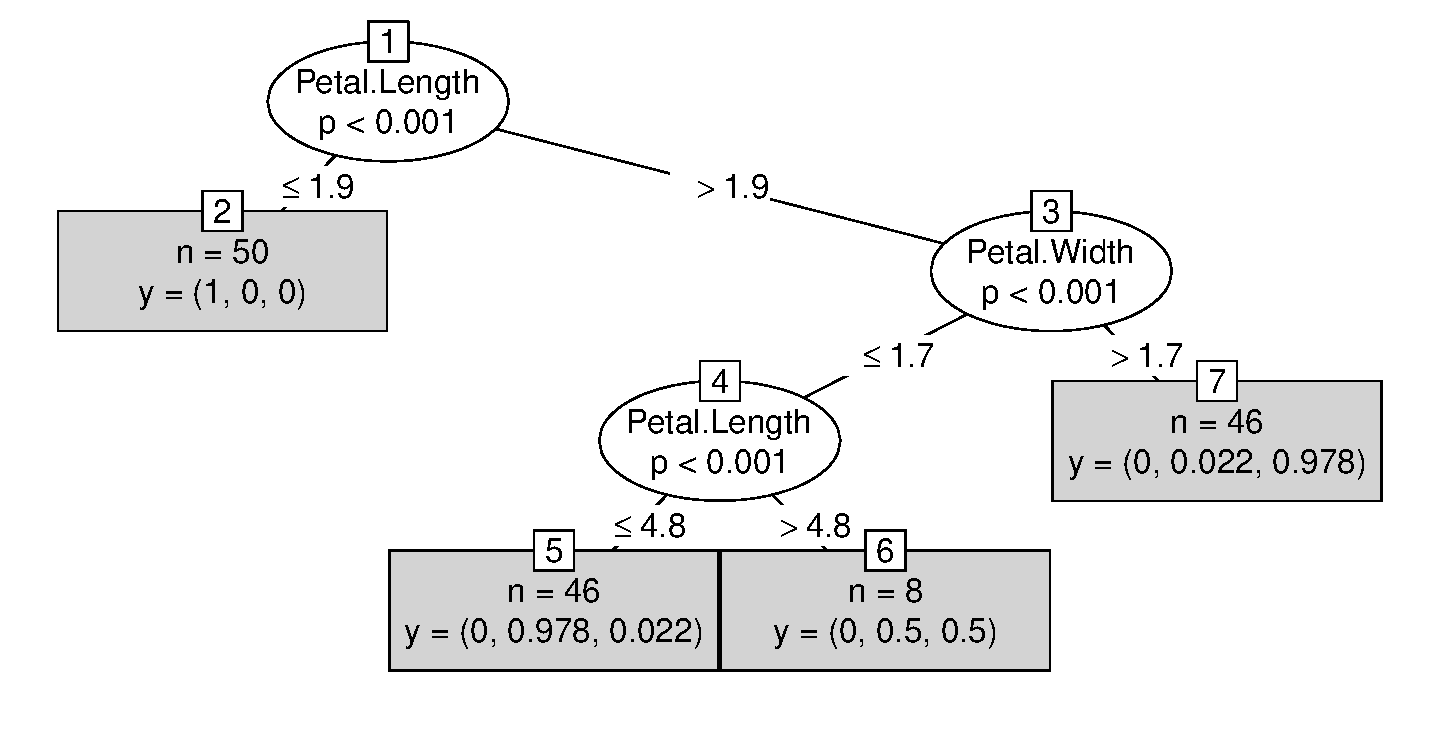
\includegraphics[width=0.8\textwidth]{dt_example.eps}
 \caption{an example of decision tree}
 \label{dt_plot_example}
\end{figure}
\end{comment}

Decision tree analysis starts with a labeled data set as the training data, because its classification ability is obtained from the learning of labeled existing data. When in the application phase, decision trees approach are always applied in conjunction with another classification method (such as clustering) to generate a reliable training model.
%like the clustering analysis methods, or other models or algorithms having to do the objects (usually customers) segmentation. 
 Common decision tree algorithms include ID3, C4.5, CART, CHAID, MARS, RainForest, BOAT, etc.  
For a review of different classification/decision tree techniques, please see \citep{dt_review}.

\subsubsection{Decision Tree Application in Enrollment Management}

\citet{dt_performance} and \citet{dt_performance1} built two similar systems to predict a student's final grade in a course by using different decision tree methods including ID3, C4.5 and CART as well as other classifier methods like Na{\"\i}ve Bayes. These  predictions were then used by instructors and academic counselors who could then provide extra help to those who are more likely to fail. This study enhanced the quality of higher education specifically in the course teaching and learning processes. \citet{dt_performance2} compared C4.5 and Random Tree in predicting the grades for a course and concluded random tree yielded higher accuracy (94.418\%) than C4.5 (88.372\%).

\citet{dt_enroll_india} proposed a new attribute selection measure function on the C4.5 method to predict the branch of engineering in which the incoming students will be enrolled. The rationale behind the proposed algorithm is that the split information never approaches zero so that the generated rule set and decision tree is stable. Then the C5.0 and artificial neural network were chosen to compare the prediction accuracy of the model and C5.0 was found to have better accuracy.

%\citet{dt_enroll_academic} designed a Cross Industry Standard Process for Data Mining (CRISP-DM) system to support the enrollment decision of a course by using students' previous academic performance. In the variable selection stage, the author used two synthetic attributes: the inherent difficulty of a testing course and the student's competence for the testing course. The problem is to classify students with similar academic performance. %In the first phase of the study, C4.5 was found to be the most effective algorithm compared to KNN and Na{\"\i}ve Bayes.

\citet{dt_graduation} chose the classification and regression tree (C\&RT) algorithm to predict the graduation rate in the Minnesota state system. Fifty-one variables were selected from over one thousand in the Integrated Postsecondary Education Data System (IPEDS). The results can provide information for students to adjust their study plans to improve school performance measures.

\subsection{Logistic Regression Tree}

It has been observed that  different subsets of students respond differently to scholarships \citep{Curs2002111,heller1999effects}. For example, students from surrounding regions would react differently from those from faraway regions. As such, it is necessary to perform a cluster analysis to separate these groups, such that each has its own logistic regression model. To achieve this goal, a logistic regression tree method is used to combine cluster analysis and logistic regression.  

Logistic regression tree is a member of the regression trees family which attempts to fit a piecewise linear logistic regression model by recursively partitioning the data and fitting a different logistic regression in each partition \citep{lotus2}. For a survey of logistic regression methods, please see \citep{harrell2013regression_book}.
	
\citet{lotus2} proposed the Logistic Tree with Unbiased Selection (LOTUS) algorithm for the automation of a logistic regression tree. In contrast to the general logistic regression tree, LOTUS allows the non-linear feature of the data sets to be modeled without transforming the variables. The method was compared with standard stepwise logistic regression on 30 real datasets and it was found that the LOTUS reduced the mean deviance by 9\% to 16\%;  For applications of the LOTUS model, please see \citep{lotus_app1,lotus_app2}. 

There have been limited studies in the use of logistic regression tree analysis in the case of enrollment management. In this study, logistic regression tree is used where variables such as education level, income, gender, and distance to school are used to separate  social-economic groups into clusters; each cluster is represented as a node in a tree and modeled through a logistic regression. The generated tree diagram is easy to interpret and the splits of nodes could also be used to identify key factors.

\subsection {Bayesian Network}
Bayesian Network is a classification method based on Bayesian probability theory.
The Bayesian probability is calculated as P(H$|$X) = P(X$|$H)  $\times$ P(H))/P(X), where X is the data sample without label; H is the hypothesis that X belongs to a class C; P(H$|$X) is the probability that the hypothesis holds the given the sample X.
P(X$|$H) is the probability of X, given the hypothesis holds. 
To classify which class C the data point belongs to, use the Bayesian method to calculate $P(C_i|X)$ and assign the data point to the class C with the maximum yield.
For more details, please see \citep{han2011data}.

%Under the enrollment prediction circumstance, P(H) will be enrolled or not enrolled, regardless of attributes like academic, income, etc; P(X) will be the probability that sample data represented by attributes is observed. P(X$|$H) is, for example, the probability that X has GPA 3.0, income high, given X is enrolled.  P(H$|$X) is the how likely the student is enrolled.

Bayesian network and other Bayesian based methods have been used in some areas in enrollment management study: 
\citet{optimization_bayesian} applied Na{\"\i}ve Bayes from Bayesian network to predict the probability of enrollment and developed an  a ensemble model to overcome highly skewed data to increase the accuracy of the prediction results.

\citet{dt_enroll_academic} used Na{\"\i}ve Bayes compared with decision tree and nearest neighbors to predict the competence of a student for a given course based on the grades. Their studies suggested that C4.5 decision tree was  the most effective algorithm in terms of prediction accuracy.
\citet{nandeshwarlearning2011} used Na{\"\i}ve Bayes to study the likelihood that students will remain for the first three years.


\section{Optimization of Financial Aid Allocation}
Though there have been a lot of mathematical models in various other industries, the use of mathematical models for enrollment management and financial aid allocation has been rather limited. 

\citet{optimization1} used a constrained optimization technique to allocate merit-based aid at a medium-sized private university. The objective of the study was to attract higher quality students, measured by combined SAT score, so as to improve the overall academic performance in the enrollment. %The constraints of the study include the availability of students in certain SAT score ranges, the total budget available, and the the enrollment limit. %The optimization models involved used the actual enrolled data from previous admission years in every level of combined SAT score. 

\citet{optimization_bayesian} presented an approach to maximize the tuition revenue through enrollment. By using a Bayesian network, the enrollment probability of each student was predicted. The accuracy of the model is 82.70\% with 10-fold cross validation. An optimization model was used to allocate the financial aid to student groups subject to capacity constraints and faculty-student ratio constraints. %The dataset for this study is very skewed, and the authors solve it by splitting the majority class (not enrolled) into groups. The authors also used an ensemble model and found that the stacking method is more suitable for the problem.


\chapter{3 Predictive Models for Enrollment and Graduation}
The first phase of the proposed approach to the solution of the optimal financial aid allocation problem is predictive models to estimate the probabilities of enrollment and of graduation, with respect to given financial aid award for each applicant. These predictive models are all based on some variant of logistic regressions and are presented here.

   
\section{Data Preparation and Visualization}
The data used in this study was provided by the institution being researched and consists of 47,932 applications that span seven years from 2006 to 2013. Out of these applications, 8,072 applications were not granted admission due to incomplete information or did not meet the admission requirement, 39,860 were granted admission. Out of the 39,860 admitted applications, 19,345 were enrolled, 20,515 were no enrolled. 

Out of the applications, 44,994 (93.8\%) of the applications are from the state of Ohio and these are the focus of this study. Financial aid awards of out-of-state and international students is quite different from the in-state students and thus are not addressed in this study. The applications from home schools (104 applicants) and applications for a satellite campus (1,796 applicants) were also removed from analysis. 

This leaves a total of 35,458 applications and the statistics of the number of applications in each year are shown in the table below. 
\begin{table}[ht]
\centering
\begin{tabular}{|c|c|c|c|c|c|c|c|}
\hline
          & 06-07 & 07-08 & 08-09 & 09-10 & 10-11 & 11-12 & 12-13 \\ \hline
Enrolled  & 2,102  & 2,201  & 2,568  & 2,541  & 2,851  & 2,985  & 2,964  \\ \hline
Not Enrolled   & 2,145  & 2,321  & 2,480  & 2,492  & 2,714  & 2,791  & 2,303  \\ \hline
\end{tabular}
\caption{The number of Applications From 2007 to 2013}
\label{enroll_sum}
\end{table}

The data fields associated with these applications can be classified into following categories: 1) academic performance related, 2) financial related, and 3) personal information. The fields in academic related category includes the applicant's SAT/ACT scores, GPA, and high school percentile; the  fields in financial  related category includes family income, expected family contribution (EFC), Pell grant; the fields in personal information category includes gender, ethnicity, high school, intended college, and intended major.

In the academic performance related fields, to normalize, the ACT score was translated into a percentile, for details on the mapping, please see \citet{ACT_percentile}.
 
In the financial related fields or variables, expected family contribution (EFC) measures an applicant's family's financial strength and is calculated according to a formula established by law. The Federal Pell Grant is a need-based grants to low-income students and is dependent on EFC. To better estimate an applicant's affordability, two more variables are introduced: total free money and out of pocket. The former defines all the awards that an applicant gets while the latter is the total out\-of\-pocket money an applicant pays. 

In the personal information related field, to better estimate the distance between applicants distance to the university, a variable was introduced that represents the distance of the applicants' high school (a character variable) into the distance from the high school to the university. 

To get an idea of the application poll, an average students has a average GPA of 3.0 and an average composite ACT score 21.2 (the state average composite ACT score is 22.0, please see \citet{mean_sat}). 60\% of the applicants are female and 40\% are male.  %The average effective family contribution is \$1400
    
To get a better picture of the applications distributions across academic measure, Table \ref{num_act_gpa}) and the number of applicants in specific GPA and ACT scores. To get a better picture of the applications distribution across geographic regions, figure presents the number of applicants across the geographic locations. 

Finally, summary statistics of the variables are presented in Appendix \ref{app A}. 


\begin{sidewaystable}[!htbp]
 \resizebox{\linewidth}{200pt}{
\begin{tabular}{@{\extracolsep{5pt}}|c|ccccccccccccccccccccccccccc|c|}
\hline
GPA/ACT     & \multicolumn{1}{c|}{9} & \multicolumn{1}{c|}{10} & \multicolumn{1}{c|}{11} & \multicolumn{1}{c|}{12} & \multicolumn{1}{c|}{13} & \multicolumn{1}{c|}{14}  & \multicolumn{1}{c|}{15}  & \multicolumn{1}{c|}{16}  & \multicolumn{1}{c|}{17}  & \multicolumn{1}{c|}{18}  & \multicolumn{1}{c|}{19}  & \multicolumn{1}{c|}{20}  & \multicolumn{1}{c|}{21}  & \multicolumn{1}{c|}{22}  & \multicolumn{1}{c|}{23}  & \multicolumn{1}{c|}{24}  & \multicolumn{1}{c|}{25}  & \multicolumn{1}{c|}{26}  & \multicolumn{1}{c|}{27}  & \multicolumn{1}{c|}{28}  & \multicolumn{1}{c|}{29}  & \multicolumn{1}{c|}{30} & \multicolumn{1}{c|}{31} & \multicolumn{1}{c|}{32} & \multicolumn{1}{c|}{33} & \multicolumn{1}{c|}{34} & 35 & Grand Total \\ \hline
1           &                        &                         &                         &                         & 1                       &                          & 2                        &                          &                          &                          &                          &                          &                          &                          &                          &                          &                          &                          &                          &                          &                          &                         &                         &                         &                         &                         &    & 3           \\ \cline{1-1} \cline{29-29} 
1.1         &                        &                         &                         &                         &                         &                          &                          &                          & 1                        &                          &                          &                          &                          &                          &                          &                          &                          &                          &                          &                          &                          &                         &                         &                         &                         &                         &    & 1           \\ \cline{1-1} \cline{29-29} 
1.2         &                        &                         &                         &                         & 1                       &                          &                          &                          &                          &                          & 1                        &                          &                          &                          &                          &                          &                          &                          &                          &                          &                          &                         &                         &                         &                         &                         &    & 2           \\ \cline{1-1} \cline{29-29} 
1.3         &                        &                         &                         & 1                       &                         &                          &                          & 1                        &                          & 1                        &                          &                          &                          &                          &                          &                          &                          &                          &                          &                          &                          &                         &                         &                         &                         &                         &    & 3           \\ \cline{1-1} \cline{29-29} 
1.4         &                        &                         &                         & 1                       &                         & 2                        &                          & 1                        &                          &                          & 2                        &                          &                          &                          &                          &                          &                          &                          &                          &                          &                          &                         &                         &                         &                         &                         &    & 6           \\ \cline{1-1} \cline{29-29} 
1.5         &                        &                         &                         & 1                       & 2                       & 2                        & 1                        & 6                        & 3                        &                          & 3                        &                          &                          &                          &                          &                          &                          & 1                        &                          &                          &                          &                         &                         &                         &                         &                         &    & 19          \\ \cline{1-1} \cline{29-29} 
1.6         &                        &                         &                         & 1                       & 4                       & 4                        & 2                        & 4                        & 4                        & 4                        & 2                        & 3                        & 2                        & 2                        & 1                        & 1                        &                          &                          &                          &                          &                          &                         &                         &                         &                         &                         &    & 34          \\ \cline{1-1} \cline{29-29} 
1.7         & 1                      &                         &                         & 2                       & 5                       & 4                        & 7                        & 3                        & 2                        & 5                        & 6                        & 1                        & 1                        & 2                        & 1                        & 2                        & 2                        & 1                        &                          &                          &                          &                         &                         &                         &                         &                         &    & 45          \\ \cline{1-1} \cline{29-29} 
1.8         &                        &                         &                         &                         & 4                       & 8                        & 5                        & 9                        & 4                        & 8                        & 4                        & 1                        & 1                        & 1                        &                          &                          &                          &                          &                          &                          &                          &                         &                         &                         &                         &                         &    & 45          \\ \cline{1-1} \cline{29-29} 
1.9         &                        & 1                       & 1                       & 2                       & 1                       & 11                       & 9                        & 7                        & 9                        & 5                        & 5                        & 5                        & 4                        & 3                        & 3                        &                          & 2                        &                          &                          &                          &                          &                         &                         &                         &                         &                         &    & 68          \\ \cline{1-1} \cline{29-29} 
2           &                        &                         &                         & 2                       & 4                       & 5                        & 7                        & 14                       & 9                        & 10                       & 7                        & 7                        & 4                        & 6                        & 3                        & 1                        & 1                        &                          &                          &                          & 1                        &                         &                         &                         &                         &                         &    & 81          \\ \cline{1-1} \cline{29-29} 
2.1         & 1                      &                         &                         & 5                       & 8                       & 7                        & 17                       & 23                       & 8                        & 14                       & 12                       & 7                        & 5                        & 5                        & 2                        &                          & 1                        & 1                        & 1                        &                          &                          & 1                       &                         &                         &                         &                         &    & 118         \\ \cline{1-1} \cline{29-29} 
2.2         &                        &                         & 1                       & 3                       & 7                       & 7                        & 11                       & 12                       & 23                       & 18                       & 13                       & 13                       & 8                        & 5                        & 2                        & 7                        & 2                        & 2                        & 1                        & 1                        & 1                        &                         &                         &                         &                         &                         &    & 137         \\ \cline{1-1} \cline{29-29} 
2.3         &                        &                         & 1                       & 3                       & 5                       & 9                        & 21                       & 21                       & 29                       & 19                       & 17                       & 15                       & 13                       & 5                        & 5                        & 7                        & 2                        & 3                        & 1                        & 2                        &                          &                         &                         &                         &                         &                         &    & 178         \\ \cline{1-1} \cline{29-29} 
2.4         &                        &                         &                         & 1                       & 4                       & 13                       & 20                       & 17                       & 30                       & 15                       & 16                       & 19                       & 21                       & 7                        & 8                        & 5                        & 2                        & 3                        & 2                        &                          &                          & 1                       &                         &                         &                         &                         &    & 184         \\ \cline{1-1} \cline{29-29} 
2.5         &                        &                         &                         & 4                       & 3                       & 13                       & 17                       & 26                       & 26                       & 22                       & 29                       & 17                       & 18                       & 11                       & 7                        & 8                        & 3                        & 3                        & 1                        & 1                        & 2                        &                         & 1                       &                         &                         &                         &    & 212         \\ \cline{1-1} \cline{29-29} 
2.6         &                        &                         & 1                       & 3                       & 4                       & 10                       & 10                       & 21                       & 26                       & 38                       & 28                       & 15                       & 13                       & 5                        & 13                       & 11                       & 5                        & 2                        & 4                        &                          & 2                        & 1                       &                         &                         & 1                       &                         &    & 213         \\ \cline{1-1} \cline{29-29} 
2.7         &                        &                         & 3                       &                         & 2                       & 7                        & 17                       & 22                       & 32                       & 27                       & 33                       & 23                       & 15                       & 15                       & 15                       & 7                        & 3                        & 2                        & 1                        & 1                        &                          & 2                       &                         &                         &                         &                         &    & 227         \\ \cline{1-1} \cline{29-29} 
2.8         &                        &                         &                         & 2                       & 4                       & 7                        & 12                       & 10                       & 28                       & 27                       & 29                       & 23                       & 19                       & 20                       & 14                       & 13                       & 4                        & 7                        & 5                        & 2                        & 1                        &                         &                         &                         & 1                       &                         &    & 228         \\ \cline{1-1} \cline{29-29} 
2.9         &                        &                         & 1                       & 2                       & 7                       & 9                        & 11                       & 25                       & 21                       & 39                       & 32                       & 40                       & 20                       & 22                       & 20                       & 15                       & 12                       & 11                       & 4                        & 1                        &                          &                         &                         &                         &                         &                         &    & 292         \\ \cline{1-1} \cline{29-29} 
3           &                        &                         &                         & 1                       & 1                       & 9                        & 9                        & 16                       & 26                       & 34                       & 33                       & 35                       & 28                       & 28                       & 26                       & 17                       & 15                       & 10                       & 3                        & 2                        & 5                        &                         & 2                       &                         &                         & 1                       &    & 301         \\ \cline{1-1} \cline{29-29} 
3.1         &                        &                         &                         & 3                       & 2                       & 6                        & 12                       & 11                       & 18                       & 36                       & 35                       & 39                       & 38                       & 18                       & 24                       & 21                       & 15                       & 11                       & 4                        & 4                        & 2                        & 1                       &                         &                         &                         &                         & 1  & 301         \\ \cline{1-1} \cline{29-29} 
3.2         &                        &                         &                         &                         &                         & 6                        & 7                        & 17                       & 19                       & 26                       & 26                       & 32                       & 29                       & 37                       & 32                       & 16                       & 16                       & 8                        & 12                       & 3                        & 8                        & 5                       & 4                       & 1                       &                         &                         &    & 304         \\ \cline{1-1} \cline{29-29} 
3.3         &                        &                         & 1                       &                         & 1                       & 4                        & 8                        & 5                        & 23                       & 22                       & 31                       & 33                       & 22                       & 34                       & 27                       & 22                       & 27                       & 19                       & 13                       & 10                       & 4                        & 3                       & 5                       &                         & 1                       & 2                       &    & 317         \\ \cline{1-1} \cline{29-29} 
3.4         &                        & 1                       &                         &                         & 1                       &                          & 3                        & 9                        & 9                        & 14                       & 21                       & 31                       & 36                       & 35                       & 30                       & 26                       & 21                       & 16                       & 10                       & 8                        & 5                        & 2                       & 3                       &                         &                         &                         &    & 281         \\ \cline{1-1} \cline{29-29} 
3.5         &                        &                         &                         &                         &                         &                          & 5                        & 5                        & 8                        & 13                       & 16                       & 23                       & 27                       & 29                       & 25                       & 29                       & 30                       & 22                       & 14                       & 11                       & 5                        & 7                       & 2                       &                         & 1                       &                         &    & 272         \\ \cline{1-1} \cline{29-29} 
3.6         &                        &                         &                         &                         &                         &                          & 2                        & 3                        & 4                        & 3                        & 22                       & 17                       & 21                       & 30                       & 37                       & 28                       & 23                       & 25                       & 18                       & 11                       & 10                       & 6                       & 1                       & 3                       & 2                       & 2                       &    & 268         \\ \cline{1-1} \cline{29-29} 
3.7         &                        &                         &                         &                         &                         & 2                        & 1                        &                          & 3                        & 7                        & 12                       & 10                       & 20                       & 20                       & 28                       & 28                       & 22                       & 25                       & 23                       & 16                       & 13                       & 5                       & 2                       & 2                       &                         & 2                       &    & 241         \\ \cline{1-1} \cline{29-29} 
3.8         &                        &                         &                         &                         &                         &                          & 2                        &                          &                          & 3                        & 8                        & 13                       & 13                       & 20                       & 18                       & 29                       & 19                       & 18                       & 27                       & 15                       & 11                       & 10                      & 3                       & 2                       & 2                       &                         &    & 213         \\ \cline{1-1} \cline{29-29} 
3.9         &                        &                         &                         &                         &                         &                          & 1                        & 2                        & 2                        & 3                        & 6                        & 6                        & 8                        & 14                       & 24                       & 26                       & 19                       & 25                       & 19                       & 17                       & 18                       & 11                      & 7                       & 5                       & 3                       & 1                       &    & 217         \\ \cline{1-1} \cline{29-29} 
4           &                        &                         &                         &                         &                         &                          &                          & 1                        &                          &                          & 2                        & 7                        & 7                        & 7                        & 20                       & 18                       & 19                       & 23                       & 23                       & 21                       & 20                       & 22                      & 9                       & 11                      & 12                      & 7                       & 2  & 231         \\ \cline{1-1} \cline{29-29} 
4.1         &                        &                         &                         &                         &                         &                          &                          &                          & 1                        &                          & 2                        & 2                        & 1                        & 3                        & 7                        & 8                        & 4                        & 6                        & 9                        & 4                        & 4                        & 6                       & 4                       & 2                       & 3                       & 1                       &    & 67          \\ \cline{1-1} \cline{29-29} 
4.2         &                        &                         &                         &                         &                         &                          &                          &                          &                          & 1                        &                          & 1                        & 2                        & 4                        & 1                        & 3                        & 5                        & 5                        & 7                        & 3                        & 4                        & 3                       & 2                       & 5                       & 1                       & 1                       &    & 48          \\ \cline{1-1} \cline{29-29} 
4.3         &                        &                         &                         &                         &                         &                          &                          &                          &                          &                          &                          &                          &                          & 1                        & 2                        & 4                        & 3                        & 2                        & 2                        & 8                        & 3                        & 3                       & 4                       & 4                       & 1                       & 1                       &    & 38          \\ \cline{1-1} \cline{29-29} 
4.4         &                        &                         &                         &                         &                         &                          &                          &                          &                          &                          &                          &                          &                          &                          &                          & 1                        & 4                        & 2                        & 3                        & 1                        & 1                        & 5                       & 2                       & 2                       & 1                       & 2                       &    & 24          \\ \cline{1-1} \cline{29-29} 
4.5         &                        &                         &                         &                         &                         &                          &                          &                          &                          &                          &                          & 1                        &                          & 1                        & 4                        &                          & 1                        & 1                        &                          & 1                        & 3                        &                         & 1                       & 2                       & 3                       &                         & 1  & 19          \\ \cline{1-1} \cline{29-29} 
4.6         &                        &                         &                         &                         &                         &                          &                          &                          &                          &                          &                          &                          &                          &                          & 1                        &                          &                          & 1                        & 1                        & 1                        &                          & 1                       &                         & 3                       & 1                       & 1                       &    & 10          \\ \cline{1-1} \cline{29-29} 
4.7         &                        &                         &                         &                         &                         &                          &                          &                          &                          &                          &                          &                          & 1                        &                          &                          &                          &                          & 1                        & 3                        & 1                        &                          &                         & 1                       & 1                       & 1                       &                         &    & 9           \\ \cline{1-1} \cline{29-29} 
4.8         &                        &                         &                         &                         &                         &                          &                          &                          &                          &                          &                          &                          &                          &                          &                          &                          &                          &                          & 1                        & 1                        &                          & 1                       &                         &                         &                         &                         &    & 3           \\ \hline
Grand Total & \multicolumn{1}{c|}{2} & \multicolumn{1}{c|}{2}  & \multicolumn{1}{c|}{9}  & \multicolumn{1}{c|}{37} & \multicolumn{1}{c|}{71} & \multicolumn{1}{c|}{145} & \multicolumn{1}{c|}{219} & \multicolumn{1}{c|}{291} & \multicolumn{1}{c|}{368} & \multicolumn{1}{c|}{414} & \multicolumn{1}{c|}{453} & \multicolumn{1}{c|}{439} & \multicolumn{1}{c|}{397} & \multicolumn{1}{c|}{390} & \multicolumn{1}{c|}{400} & \multicolumn{1}{c|}{353} & \multicolumn{1}{c|}{282} & \multicolumn{1}{c|}{256} & \multicolumn{1}{c|}{212} & \multicolumn{1}{c|}{146} & \multicolumn{1}{c|}{123} & \multicolumn{1}{c|}{96} & \multicolumn{1}{c|}{53} & \multicolumn{1}{c|}{43} & \multicolumn{1}{c|}{34} & \multicolumn{1}{c|}{21} & 4  & 5260        \\ \hline
\end{tabular}}
\caption{Number of Applicants vs GPA/ACT in 2012-2013}
\label{num_act_gpa}
\end{sidewaystable}

%  cost of attendance; the student's enrollment status; and whether the student attends for a full academic year or less. The Federal Pell Grant data used in the study was derived follow by \citep{EFC_Pell}.

\section{Logistic Regression Models}
Logistic regression is a popular method when predicting a dichotomous outcome variable. In the case of prediction of enrollment, the response variable has two levels (yes and no). The output of logistic regression model is the probability of the enrollment levels; for example, a probability of 70\% of enrollment (yes) for an applicant with GPA 2.5, ACT 28, given say a \$1000 scholarships. 

Because of the fact that the probability of enrollment $p(x)$ must fall in $[0,1]$, a regular linear regression is unsuitable as the regression function is not bounded. To resolve this issue, the ratio, called the odds of success, defined as  $\frac{p(x)}{1-p(x)}$,  is used to form a regression and and a logistic function is defined as:
\begin{equation}
\ensuremath{\log\frac{p(x)}{1-p(x)}=\beta_0+\beta_1 x_1+\beta_2 x_2 +\ldots+\beta_k x_k}
\end{equation}
The probability of enrollment can thus be rewritten as:
\begin{equation}
	p(x)=\frac{e^{\beta_0+\beta_1 x_1+\beta_2 x_2 +\ldots+\beta_i x_i}}{1+e^{\beta_0+\beta_1 x_1+\beta_2 x_2 +\ldots+\beta_i x_i}}%=\frac{1}{1+e^{-(\beta_0+\beta_0+\beta_1 x_1+\beta_2 x_2 +\ldots+\beta_k x_k)}}
\end{equation}
Here, $\beta_0$ is the intercept and $\beta_1 \ldots \beta_i$ are parameters for corresponding variable $x_i$.  Here $x_i$ could be either continuous variables such as GPA or  ACT, or categorical variables such as gender, ethnicity or region. 

\begin{comment}
This function will always generate an S-shape curve as shown below:
\begin{figure}[ht]
   \centering
 \includegraphics[scale=0.5]{pic/LR_EXAMPLE}
 \caption{Logistic Regression Example}
\end{figure}
\end{comment}

\begin{comment}
\textbf{An example of a cumulative distribution function plot of logistic regression is shown below, which has a "S" shaped curves between 0 and 1.  shuai, in the figure, you said a=0, b=.5, what does this mean? }
\begin{figure}[h!]
   \centering
\includegraphics[width=0.4\textwidth]{LR.png}
 \caption{"S" shaped curve in logistic regression}
\end{figure}
\end{comment}

Parameters $\beta_0$ and $\beta_i$ are estimated by the maximum likelihood estimation.
\begin{equation}
	\ell(\beta_0,\ldots \beta_i) = \prod_{i:y_i=1} p(x_i)  \prod_{i^{'}:y_i{^{'}=0}} (1-p(x_{i^{'}}))
\end{equation}
For details on the derivation of the parameter estimations, please see \citet{hosmer2004applied}.

\subsection{A Logistic Regression Model}

The baseline model is a general linear logistic regression model.  Before the model is presented, multicolinearity, or collinearity among variables is first explored.     

\subsubsection{Collinearity }

Multicollinearity or collinearity is a phenomenon in which two or more predictor variables in a multiple regression model are highly correlated. In this situation the coefficient estimates of the multiple regression may change erratically in response to small changes in the model or the data.  \citep{belsley2005regression,Midi2010}.

A common method to detect collinearity is to examine the correlation matrix.  In the building of the logistic regression model, the following variables were used GPA, ACT, HS.PERCENTILE, UNEMPLOYMENT.INDEX, PELL.GRANT, SCHOLARSHIP, APP.COLLEGE, DISTANCE.BIN, HS.COUNTY.TIER, UNDERREPRESENTED, ETHNICITY.  The correlation matrix  of the continuous variables is presented in Table \ref{correlation_matrix}. % and scatter plot among these variables are shown in Appendix B. \textbf{shuai} 

\begin{sidewaystable}[!htbp]
\small
\resizebox{\linewidth}{130pt}{
\begin{tabular}{@{\extracolsep{4pt}} lcccccccccc}
	
\\[-1ex]\hline 
\hline \\[-1.8ex] 
                   & GPA            & ACT    & \begin{tabular}[c]{@{}c@{}}HS.\\ PERCENTILE\end{tabular} & \begin{tabular}[c]{@{}c@{}}SCHOLAR-\\ SHIP\end{tabular} & \begin{tabular}[c]{@{}c@{}}PELL.\\ GRANT\end{tabular} & \begin{tabular}[c]{@{}c@{}}TOTAL.\\ FREE.MONEY\end{tabular} & \begin{tabular}[c]{@{}c@{}}OUT.OF.\\ POCKET\end{tabular} & \begin{tabular}[c]{@{}c@{}}DISTANCE.\\ NUM\end{tabular} & \begin{tabular}[c]{@{}c@{}}UNEMPLOYMENT.\\ INDEX\end{tabular} \\
                   \\ \hline
\hline \\[-1.8ex] 
                   
GPA                & 1              & 0.596  & \textbf{0.884}                                           & 0.612                                                   & -0.190                                                & 0.159                                                       & -0.164                                                   & -0.017                                                  & -0.018                                                        \\
ACT                & 0.596          & 1      & 0.469                                                    & 0.586                                                   & -0.275                                                & 0.069                                                       & -0.070                                                   & -0.039                                                  & 0.005                                                         \\
HS.PERCENTILE      & \textbf{0.884} & 0.469  & 1                                                        & 0.594                                                   & -0.060                                                & 0.266                                                       & -.0271                                                   & 0.011                                                   & -0.010                                                        \\
SCHOLARSHIP        & 0.612          & 0.586  & 0.594                                                    & 1                                                       & 0.025                                                 & 0.456                                                       & -0.456                                                   & 0.031                                                   & 0.010                                                         \\
PELL.GRANT         & -0.190         & -0.275 & -0.060                                                   & 0.025                                                   & 1                                                     & \textbf{0.845}                                              & \textbf{-0.830}                                          & 0.023                                                   & 0.132                                                         \\
TOTAL.FREE.MONEY   & 0.159          & 0.069  & 0.266                                                    & 0.456                                                   & \textbf{0.845}                                        & 1                                                           & \textbf{-0.987}                                          & 0.037                                                   & 0.124                                                         \\
OUT.OF.POCKET      & -0.164         & -0.070 & -0.271                                                   & -0.456                                                  & \textbf{-0.830}                                       & \textbf{-0.987}                                             & 1                                                        & -0.039                                                  & -0.045                                                        \\
DISTANCE.NUM       & -0.017         & -0.039 & 0.011                                                    & 0.031                                                   & 0.023                                                 & 0.037                                                       & -0.039                                                   & 1                                                       & -0.010                                                        \\
UNEMPLOYMENT.INDEX & -0.018         & 0.005  & -0.010                                                   & 0.010                                                   & 0.132                                                 & 0.124                                                       & -0.045                                                   & -0.010                                                  & 1 \\ 
\hline \\[-1.8ex]                                                            
\end{tabular}}
\caption{Pearson Correlation Matrix of all Numeric Variables} 
  \label{correlation_matrix} 
\end{sidewaystable}


As can be seen from Table, according to \citep{hinkle2003applied}, there exists a very high correlation ( $0.9$ to $1$ or $-0.9$ to $-1$ ) between the monetary variables such as between Out of Pocket and Total Free Money, and high correlation( $0.7$ to $0.9$ or $-0.7$ to $-0.9$ ) between GPA and HS.PERCENTILE, and between PELL Grant, Out of Pocket and Total Free Money.   Though this result is not surprising, and collinearity does not reduce the predictive power or reliability of the model as a whole, collinearity it does affect calculations regarding individual predictors and cause unstable estimates of coefficients in regression analysis. That is, a multiple regression model with correlated predictors can indicate how well the entire bundle of predictors predicts the outcome variable, but it may not give valid results about any individual predictor, or about which predictors are redundant with respect to others.
  
\subsubsection{Variable Selection}
In regression analysis with multiple variables, strategies have been designed to select the best variables in the model. There are several approaches for variable selection and stepwise regression is one of the most popular semi-automated procedures \citep{han2011data}. 

Stepwise variable selection include backward elimination, forward selection and bidirectional elimination. A backward stepwise regression, for example, works as follows: a) start with the model containing all potential predictors; b) try subtracting one predictor at a time. Keeping the model if it improves the measure of predictive accuracy; and c) iterate until no further improvement.

Several criterion have been proposed in variable selection to determine which model works best. For logistic regression the most common criteria used in  are BIC, AIC, AICc.  AIC (Akaike information criterion) is defined for a large class of models fit by maximum likelihood and in logistic regression, AIC is calculated as:
\begin{equation}
	AIC= -2 \times \ln(likelihood) + 2k
\end{equation}
where $k$ is the number of variables included in that model. For details, please see  \citep{han2011data}. 
	
In an enrollment model, say with 13 predictor variables, to get the optimal model, a brute-force approach would have to evaluate $2^{13}$ possible models.  The stepwise variable selection evaluates only a limited number of models and presents a heuristic solution to the problem in a fraction of time.  

In our implementation, a backward stepwise procedure was adopted and the detailed backward stepwise selection process is presented in Table \ref{back}. In the table, the ``steps" column represents the number of iterations; the ``model" column represents the model in each iteration; the ``AIC" column represents the AIC value.  As can be seen, the process started with a full model with all of the predictor variables and continued to seek models with lower AIC.

\begin{sidewaystable}[!htbp]
 \resizebox{\linewidth}{150pt}{
\begin{tabular}{@{\extracolsep{4pt}} |c|l|l|l|}
\hline
\multicolumn{1}{|c|}{Step} & \multicolumn{1}{c|}{Model}   & \multicolumn{1}{c|}{\begin{tabular}[c]{@{}c@{}}Variables\\ Dropped\end{tabular}}                                                                                                                                                                                                               & \multicolumn{1}{c|}{AIC}      \\ \hline
1                          & \begin{tabular}[c]{@{}l@{}}MATRICULATION $\sim$ GPA + ACT + HS.PERCENTILE + OUT.OF.POCKET + \\ UNEMPLOYMENT.INDEX + SCHOLARSHIP + APP.COLLEGE +\\ DISTANCE.NUM + DISTANCE.BIN + HS.COUNTY.TIER +\\ UNDERREPRESENTED + ETHNICITY +GENDER + PELL.GRANT\end{tabular} &   & \multicolumn{1}{c|}{39337.41} \\ \hline
2                          & \begin{tabular}[c]{@{}l@{}}MATRICULATION $\sim$ GPA + ACT + HS.PERCENTILE + OUT.OF.POCKET +\\ UNEMPLOYMENT.INDEX + SCHOLARSHIP + APP.COLLEGE + \\ DISTANCE.NUM + DISTANCE.BIN + HS.COUNTY.TIER + \\ ETHNICITY + GENDER + PELL.GRANT\end{tabular}       &UNDERREPRESENTED          & 39335.43                      \\ \hline
3                          & \begin{tabular}[c]{@{}l@{}}MATRICULATION $\sim$ GPA + ACT + HS.PERCENTILE + OUT.OF.POCKET + \\ UNEMPLOYMENT.INDEX +SCHOLARSHIP + APP.COLLEGE + \\ DISTANCE.NUM + DISTANCE.BIN + HS.COUNTY.TIER +\\  ETHNICITY + GENDER\end{tabular}      &UNDERREPRESENTED,  PELL.GRANT                         & \multicolumn{1}{c|}{39333.99} \\ \hline
4                          & \begin{tabular}[c]{@{}l@{}}MATRICULATION $\sim$ GPA + ACT + HS.PERCENTILE + OUT.OF.POCKET +\\ UNEMPLOYMENT.INDEX +SCHOLARSHIP + APP.COLLEGE + \\ DISTANCE.NUM + DISTANCE.BIN + HS.COUNTY.TIER + ETHNICITY\end{tabular}                     &UNDERREPRESENTED,  PELL.GRANT, GENDER                     & 39333.01                      \\ \hline
5                          & \begin{tabular}[c]{@{}l@{}}MATRICULATION $\sim$ GPA + ACT + HS.PERCENTILE + OUT.OF.POCKET +\\ UNEMPLOYMENT.INDEX +SCHOLARSHIP + APP.COLLEGE + \\ DISTANCE.BIN + HS.COUNTY.TIER +ETHNICITY\end{tabular} 
& UNDERREPRESENTED, PELL.GRANT, GENDER,  DISTANCE.NUM               & 39332.06                      \\ \hline
\end{tabular} }
\caption{Backward Stepwise Selection Process}
\label{back}
\end{sidewaystable}

%\subsubsection{Residual Analysis}

\subsubsection{Training, Testing and Results for Enrollment Data}
The data from academic years from 2008-2009 to 2011-2012 is used as training data  and the data from academic year 2012-2013 as testing data. The training data has 30,083 entries and the testing data has 5,260 entries. The general logistic regression model derived from the backward stepwise selection was used as the baseline model. 

If it is determine that $p(x) \geq 0.5$, then enrollment;  otherwise, not enroll, then the accuracy and performance indicator of the model is presented in Table  \ref{accuracy_model}.  %\textbf{ Please explain this table }. \textbf{
The accuracy of the logistic regression model is 61.9 while the AUC is 0.658, and the data is not biased towards positive or negative class as shown in \citep{optimization_bayesian}. %}

% Please add the following required packages to your document preamble:
% \usepackage{multirow}
\begin{table}[!ht]
\centering
\begin{threeparttable}
\begin{tabular}{|l|c|c|l|l|l|}
\hline
\multicolumn{1}{|c|}{Model}          & \multicolumn{1}{l|}{AUC} & Accuracy                & Enrolled                                                          & \begin{tabular}[c]{@{}l@{}}True Positive/\\ Negative Rate\end{tabular} & \begin{tabular}[c]{@{}l@{}}False Positive/\\ Negative Rate\end{tabular} \\ \hline
\multirow{2}{*}{Logistic Regression} & \multirow{2}{*}{0.658}   & \multirow{2}{*}{0.619 \tnote{*} } & \multirow{2}{*}{\begin{tabular}[c]{@{}l@{}}Yes\\ No\end{tabular}}	 & 0.646                 & 0.414                                                                      \\ \cline{5-6} &  &   &  & 0.586            & 0.354                                                                      \\ \hline  
\end{tabular}
\begin{tablenotes}\footnotesize
\item[*] 95\% CI
\end{tablenotes}
\end{threeparttable}
\caption{Accuracy of Enrollment Prediction from Logistic Regression Model }
\label{accuracy_model}
\end{table}

\begin{comment}
	


\begin{table}[!ht]
\centering
\begin{threeparttable}
\begin{tabular}{|l|c|c|l|l|l|}
\hline
\multicolumn{1}{|c|}{Model}          & \multicolumn{1}{l|}{AUC} & Accuracy                & Enrolled                                                          & \begin{tabular}[c]{@{}l@{}}True Positive/\\ Negative Rate\end{tabular} & \begin{tabular}[c]{@{}l@{}}False Positive/\\ Negative Rate\end{tabular} \\ \hline
\multirow{2}{*}{Logistic Regression} & \multirow{2}{*}{---}   & \multirow{2}{*}{--- \tnote{*} } & \multirow{2}{*}{\begin{tabular}[c]{@{}l@{}}Yes\\ No\end{tabular}}	 & -----               & ---                                                                      \\ \cline{5-6} &  &   &  & ----         & ---- \\ \hline  
\end{tabular}
\begin{tablenotes}\footnotesize
\item[*] 95\% CI
\end{tablenotes}
\end{threeparttable}
\caption{Accuracy of Graduation Prediction from Logistic Regression Model }
\label{accuracy_model}
\end{table}
\end{comment}

\begin{comment}
\textbf{Rather than the use of 0.5 as the discrimination threshold,  a receiver operating characteristic (ROC) curve is used by plotting the true positive rate (TPR) against the false positive rate (FPR) at various threshold settings, }  let the discrimination threshhold be $\theta$, which ranges from 0 to 1,  the ROC curve is presented in Fig \ref{log_ROC}:


\textbf{Here, for example, when $\theta = 0.5$, it shows that ....etc.   when $\theta = 0.5$, it shows that ....etc. ...}

\textbf{what does the ROC curve tell you, other than accuracy? }

 \begin{figure}[!ht]
   \centering
 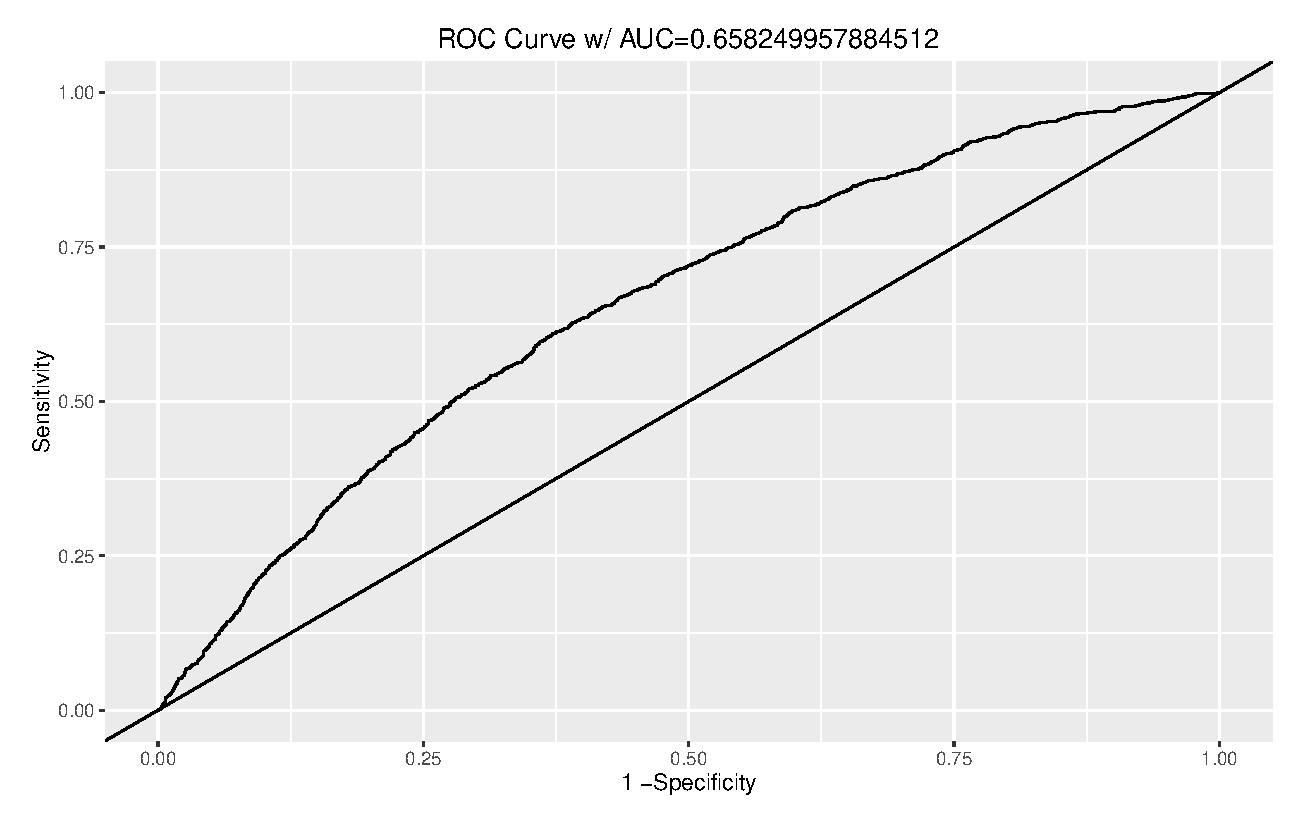
\includegraphics[scale=0.70]{pic/model_roc.eps}
 \caption{ROC Curve of the Logistic Model }
 \label{log_ROC}
\end{figure}

\end{comment}

\subsection{Logistic Regression Tree Model, Support Vectors Machines Models, and Neural Network }
A logistic regression tree model extends the baseline logistic regression model and uses a \textit{divide and conquer} strategy to divide  a complex set of data into many subsets such that a linear logistic regression model adequately fits the data in each subset. The division of the data into subset is performed recursively, one variable at a time, and results in the partitions as a binary decision tree \citep{harrell2013regression_book}. 

The logistic tree with unbiased selection (LOTUS) algorithm \citep{lotus2}  is selected in this research for the automation of a logistic regression tree. LOTUS allows the nonlinear feature of the data sets to be modeled without transforming the variables and compares favorable with standard stepwise logistic regression \citep{lotus_app1,lotus_app2}. %The LOTUS implementation of the logistic regression tree is used in this analysis; for details, please see \citep{lotus2}.


\subsection{Results of Various Models on Enrollment and Graduation Predication}
\subsubsection{Results on Enrollment and Graduation Predication}

In this research, two logistic regression trees are being constructed: one for enrollment, one for graduation.  In the construction of these tree models, the variables used in these two tree models and their role in the tree models are listed in the table below. Here, D represents the dependent variable, S is used as a numerical variable to split the tree, C represents categorical variables to split the tree, F represents the decision variables used in the logistic regression function at the tree node.  The model accuracy for the logistic regression trees are presented in the Tables \ref{accuracy_model_enroll}. %\textbf{removed  HS.COUNTY.TIER} and \ref{accuracy_model_graduation}. 

\begin{table}[h]
\centering
\begin{tabular}{|l|c|c|c|c|}
\hline
 %& \multicolumn{2}{c|}{Variables} & \multicolumn{2}{c|}{Variables} \\ \hline
\multicolumn{1}{|c|}{\multirow{2}{*}{Column}} & \multicolumn{2}{c|}{Enrollment}                            & \multicolumn{2}{c|}{Graduation}                            \\ \cline{2-5} 
\multicolumn{1}{|c|}{}                        & Name                          & Type                     & Name                          & Type                     \\ \hline
1                                             & Enrolled                      & D                        & Enrolled                      & X                        \\ \hline
2                                             & GPA                           & S                        & GPA                           & S                        \\ \hline
3      & Tier   & C    &   Tier   & C    \\ \hline
4    & Raider     & C   &   Raider  & C   \\ \hline
5   & ACT    & S  &  ACT    & S     \\ \hline
6   & Underrepresented & C     & Underrepresented    & C   \\ \hline
7    & Gender   & C   &  Gender  & C   \\ \hline
8   & Ethnicity    & C     & Ethnicity   & C      \\ \hline
9   & Scholarship(\$)    & F   & Scholarship(\$)     & F    \\ \hline
10  & Scholarship(\%)   & F     & Scholarship(\%)     & F  \\ \hline
11  & Estimated Tuition  & S    & Estimated Tuition  & S   \\ \hline
12  & Graduate   & X     &   Graduate        & D         \\ \hline
\end{tabular}
\caption{Variables Used in The Model}
\end{table}

% Please add the following required packages to your document preamble:
% \usepackage{multirow}
\begin{table}[!ht]
\centering
\begin{threeparttable}
\begin{tabular}{|l|c|c|l|l|l|}
\hline
\multicolumn{1}{|c|}{Model}          & \multicolumn{1}{l|}{AUC} & Accuracy                & Enrolled                                                          & \begin{tabular}[c]{@{}l@{}}True Positive/\\ Negative Rate\end{tabular} & \begin{tabular}[c]{@{}l@{}}False Positive/\\ Negative Rate\end{tabular} \\ \hline
\multirow{2}{*}{Logistic Regression Tree} & \multirow{2}{*}{0.618}   & \multirow{2}{*}{0.62 \tnote{*} } & \multirow{2}{*}{\begin{tabular}[c]{@{}l@{}}Yes\\ No\end{tabular}}	 & 0.65                & 0.414                                                                      \\ \cline{5-6} &  &   &  & 0.586          & 0.35 \\ \hline  
\end{tabular}
\begin{tablenotes}\footnotesize
\item[*] 95\% CI
\end{tablenotes}
\end{threeparttable}
\caption{Accuracy of Enrollment Prediction from Logistic Regression Tree Model }
\label{accuracy_model_enroll}
\end{table}

\subsubsection{Results on Graduation Predication}

\begin{comment}
	

% Please add the following required packages to your document preamble:
% \usepackage{multirow}
\begin{table}[!ht]
\centering
\begin{threeparttable}
\begin{tabular}{|l|c|c|l|l|l|}
\hline
\multicolumn{1}{|c|}{Model}          & \multicolumn{1}{l|}{AUC} & Accuracy                & Enrolled                                                          & \begin{tabular}[c]{@{}l@{}}True Positive/\\ Negative Rate\end{tabular} & \begin{tabular}[c]{@{}l@{}}False Positive/\\ Negative Rate\end{tabular} \\ \hline
\multirow{2}{*}{Logistic Regression Tree} & \multirow{2}{*}{---}   & \multirow{2}{*}{--- \tnote{*} } & \multirow{2}{*}{\begin{tabular}[c]{@{}l@{}}Yes\\ No\end{tabular}}	 & ----               & ----                                                                     \\ \cline{5-6} &  &   &  & ----            & ---- \\ \hline  
\end{tabular}
\begin{tablenotes}\footnotesize
\item[*] 95\% CI
\end{tablenotes}
\end{threeparttable}
\caption{Accuracy of Graduation Prediction from Logistric Regression Tree Model }
\label{accuracy_model_graduation}
\end{table}
\end{comment}

Preliminary experience with other logistic based models such as support vector machines, neural network,  suggest similar accuracy results. The accuracy of prediction from support vector machines and nerual network results are shown in the tables \ref{accuracy_model_enrollment_svm} %and  \ref{accuracy_model_graduation_svm}%,
  %and the accuracy of prediction from neural network are shown in tables \ref{accuracy_model_enrollment_nn} and 
  %\ref{accuracy_model_graduation_nn}.

\begin{table}[!ht]
\centering
\begin{threeparttable}
\begin{tabular}{|l|c|c|l|l|l|}
\hline
\multicolumn{1}{|c|}{Model}          & \multicolumn{1}{l|}{AUC} & Accuracy                & Enrolled                                                          & \begin{tabular}[c]{@{}l@{}}True Positive/\\ Negative Rate\end{tabular} & \begin{tabular}[c]{@{}l@{}}False Positive/\\ Negative Rate\end{tabular} \\ \hline
\multirow{2}{*}{Support Vector Machine} & \multirow{2}{*}{0.612}   & \multirow{2}{*}{0.608 \tnote{*} } & \multirow{2}{*}{\begin{tabular}[c]{@{}l@{}}Yes\\ No\end{tabular}}	 & 0.531               & 0.306                                                                     \\ \cline{5-6} &  &   &  & 0.694            & 0.469 \\ \hline  

\multirow{2}{*}{Neural Network} & \multirow{2}{*}{0.611}   & \multirow{2}{*}{0.616 \tnote{*} } & \multirow{2}{*}{\begin{tabular}[c]{@{}l@{}}Yes\\ No\end{tabular}}	 & 0.647               & 0.425                                                                     \\ \cline{5-6} &  &   &  & 0.575            & 0.353 \\ \hline  

\end{tabular}
\begin{tablenotes}\footnotesize
\item[*] 95\% CI
\end{tablenotes}
\end{threeparttable}
\caption{Accuracy of Enrollment Prediction from Support Vector Machine Model and Neural Network}
\label{accuracy_model_enrollment_svm}
\end{table}


\begin{comment}
\begin{table}[!ht]
\centering
\begin{threeparttable}
\begin{tabular}{|l|c|c|l|l|l|}
\hline
\multicolumn{1}{|c|}{Model}          & \multicolumn{1}{l|}{AUC} & Accuracy                & Enrolled                                                          & \begin{tabular}[c]{@{}l@{}}True Positive/\\ Negative Rate\end{tabular} & \begin{tabular}[c]{@{}l@{}}False Positive/\\ Negative Rate\end{tabular} \\ \hline
\multirow{2}{*}{Support Vector Machine} & \multirow{2}{*}{---}   & \multirow{2}{*}{--- \tnote{*} } & \multirow{2}{*}{\begin{tabular}[c]{@{}l@{}}Yes\\ No\end{tabular}}	 & ----               & ----                                                                     \\ \cline{5-6} &  &   &  & ----            & ---- \\ \hline  
\end{tabular}
\begin{tablenotes}\footnotesize
\item[*] 95\% CI
\end{tablenotes}
\end{threeparttable}
\caption{Accuracy of Graduation Prediction from Support Vector MachineModel }
\label{accuracy_model_graduation_svm}
\end{table}
\end{comment}

%\begin{comment}
The prediction of graduate prediction was done in the similar fashion. The comparison metrics of the graduation model are shown in Table \ref{grad_accuracy_table}:

\begin{table}[!ht]
\centering
\begin{threeparttable}
\begin{tabular}{|l|c|c|l|l|l|}
\hline
\multicolumn{1}{|c|}{Model}    & \multicolumn{1}{l|}{AUC} & Accuracy                & Graduated                                                          & \begin{tabular}[c]{@{}l@{}}True Positive/\\ Negative Rate\end{tabular} & \begin{tabular}[c]{@{}l@{}}False Positive/\\ Negative Rate\end{tabular} \\ \hline
\multirow{2}{*}{Logistic Regression} & \multirow{2}{*}{0.79}   & \multirow{2}{*}{0.74 \tnote{*} } & \multirow{2}{*}{\begin{tabular}[c]{@{}l@{}}Yes\\ No\end{tabular}}	 & 0.8               & 0.41                                                                     \\ \cline{5-6} &  &   &  & 0.59            & 0.2 \\ \hline  

\multirow{2}{*}{Logistic Regression Tree} & \multirow{2}{*}{0.76}   & \multirow{2}{*}{0.739 \tnote{*} } & \multirow{2}{*}{\begin{tabular}[c]{@{}l@{}}Yes\\ No\end{tabular}}	 & 0.88               & 0.57                                                                    \\ \cline{5-6} &  &   &  & 0.43            & 0.12 \\ \hline  

\end{tabular}
\begin{tablenotes}\footnotesize
\item[*] 95\% CI
\end{tablenotes}
\end{threeparttable}
\caption{Accuracy of Graduation Prediction from Logistic Regression and Logistic Regression Tree}
\label{grad_accuracy_table}
\end{table}

Due to space limitations, Details of these advance models such as support vector machine and neural network are not represented in the proposal. To further develop these models to increase the prediction accuracy is the focus of the rest of the study. 

\section{Model Results}

The predictions of enrollment probabilities for six applications with different levels of scholarship awards are listed in table \ref{prediction_sample}. Here, the concatenate string under ``student'' represents the characteristic of the student. For example, student ``2.9-Tier1-19-White'' represents an application from a student with a high school GPA of 2.9,ACT score of 19, lives in Tier 1 region, and is of white ethnicity.   the number represents the probabilities of enrollment in percentage of the corresponding scholarship awards, which spans from 0 to 10,000. 

\begin{table}[ht]
\centering
 \small
 \setlength\tabcolsep{4pt}
    \begin{tabular}{|c|c|c|c|c|c|c|c|c|c|c|c|}
    \hline
    \multicolumn{12}{ |c| }{GPA 2.9, ACT 19 }  \\ \hline
    & Student               & 0       & 1000    & 2000    & 3000    & 4000    & 5000    & 6000    & 7000    & 8000    & 10000   \\ \hline
    1& 2.9-Tier1-19-White    & 59.55 & 64.63 & 69.39 & 73.77 & 77.73 & 81.24 & 84.31 & 86.96 & 89.22 & 91.72 \\ \hline
    2& 2.9-Tier5-19-White    & 36.96 & 40.20 & 43.53 & 46.92 & 50.34 & 53.75 & 57.13 & 60.45 & 63.67 & 69.74 \\ \hline
     \multicolumn{12}{ |c| }{GPA 3.3, ACT  25 }   \\ \hline
    3& 3.3-Tier1-25-Hispanic & 23.80 & 27.44 & 31.42 & 35.69 & 40.20 & 44.88 & 49.65 & 54.43 & 59.13 & 67.97 \\ \hline
    4& 3.3-Tier1-25-White    & 55.60 & 59.32 & 62.94 & 66.42 & 69.72 & 72.84 & 75.75 & 78.43 & 80.90 & 85.17 \\ \hline
    \multicolumn{12}{ |c| }{GPA 3.8,ACT 28 }     \\ \hline
    5& 3.8-Tier1-28-White    & 42.29 & 46.05 & 49.85 & 53.65 & 57.41 & 61.08 & 64.63 & 68.03 & 71.25 & 77.07 \\ \hline
    6& 3.8-Tier4-28-White    & 20.54 & 22.87 & 25.37 & 28.05 & 30.89 & 33.89 & 37.02 & 40.26 & 43.60 & 50.41 \\ \hline
    \end{tabular}
\caption{ Prediction Of Enrollment of Applicants Under Different Levels of  Scholarships}
\label{prediction_sample}
\end{table}

Several interesting observations can be seen from these predictions, a) as GPA increases, the probability of enrollment decreases; b) local students (Tier 1) have a larger probability of enrollment than distance students (other tiers); c) as financial aid increases, the probability of enrollment increases; yet increase in probability with respect to scholarship is different among different student groups. 

Comparison of students 1 an 2, though both students have the same GPA and ACT score and are of the same ethnicity, student 1 who lives in tier 1 has a much higher probability of enrollment than that of student 2 who live in tier 5. 

Comparison of students 1 an 5, though both students lives in the same region, tier 1, are of the same ethnicity, student 1, who has a GPA of 2.9, ACT of 19, has a higher probability of enrollment than student 5, who has a GPA of 3.8 and ACT of 28.

Comparison of students 3 and 4, though both students lives in the same region, tier 1, have the same GAP of 3.3 and ACT of 25, student 1, who is of White ethnicity, has a higher probability of enrollment than student 5, who is of Hispanic ethnicity.

In all these cases, the probability of enrollment increases with the increase of scholarship awards. Though these observations are not surprising, accurate quantitative prediction of these probabilities are essential to the allocation of scholarship. 

However, it has to mention that the prediction of these probabilities alone has not yet solve the fundamental problems for the enrollment management team of any higher institution;  The optimal allocation of the scholarship to optimize an institution's revenue, and the formation of concrete policies and action plans needs to be solved. This is the second part of the research and is addressed in the following sections.


\chapter{4 Optimal Allocation of Financial Aid }

The study of response to scholarship, though provided much insights to the behavior of the students in responding to scholarship, has not addressed fundamentally the allocation of limited financial aid to students.  

For example, it is easy to see that local students requires less money while students in far-away regions may require more money, it is still puzzling as a) should we allocate the money to local students as they are our peanut and butter students and requires less money or b) should we allocate the money to far-away students as local students will come anyway? The solution to these problems requires the solution of an optimization problem to optimally allocate the financial aid.  This is the second part of the overall approach and is addressed in this chapter. 

\section{The Financial Aid Optimization Model}

\noindent Given a set of applicants and their probabilities of enrollment and of graduation with respect to different levels of financial aids, the optimization problem to be solved is to determine the financial aid to each applicant so as to to maximize the revenue. This is referred as the financial aid allocation problem. 

In the development of the model, the following notation is used. 
%------ define the list of set, variables, parameters ------------------------------------
\newenvironment{conditions*}
  {\par\vspace{\abovedisplayskip}\noindent
   \tabularx{\columnwidth}{>{$}l<{$} @{}>{${}}c<{{}$}@{} >{\raggedright\arraybackslash}X}}
  {\endtabularx\par\vspace{\belowdisplayskip}}
 % http://tex.stackexchange.com/questions/95838/how-to-write-a-perfect-equation-parameters-description
%---------------------------------------------------------------------  
\begin{conditions*}
\noindent\textbf{Sets}\\
I  \mbox{\qquad \qquad} &   & set of applicants,  indexed by $i$ and $j$ \\
M     &   & set of  different levels of financial awards, indexed by $m $\\
       &   &   $m \in  M = \{ 0,1000, 2000, \ldots ,8000\} $
\end{conditions*}
\vspace{-0.3in}

\begin{conditions*}
\textbf{Parameters}\\
p^e_{im}  & & probability of enrollment for applicant $i$, if given award $m$ \\
p^g_{im}    & & probability of graduation for applicant $i$, if given award $m$\\
d(i,j)         & & 1 if applicant $i$ dominates applicant $j$; 0 otherwise.\\
B                & & total budget for financial aid\\
A_m              & &  monetary value of award $m$\\
T_i             & & tuition paid by applicant $i$\\
SSI_i     & & government compensation for applicant $i$ when he/she graduates\\
N_i    & & expected number of years student $i$ stays at the institution  \\  
\textbf{Variables}\\
x_{im}           & & whether a financial award $m$ is allocated to applicant $i$ or not\\ 
\end{conditions*}

\hspace{-0.5cm}\textbf{Objective}
\begin{align}
\max \quad
& \sum_{i\in I} \sum_{m\in M} x_{im}\cdot p^e_{im}\cdot(T_i-A_m)\cdot N_{im}+
\sum_{i\in I} \sum_{m\in M} x_{im}\cdot p^e_{im} \cdot p^g_{im}\cdot SSI_i  \label{objective}
\end{align}

\hspace{-0.55cm}\textbf{Subject to}
\begin{align}
\sum_{m \in M}x_{im}=1 &&	\forall i\in I \label{constraint:1}  \\
\sum_{i \in I} \sum_{m\in M} x_{im}\cdot p^e_{im}\cdot A_m\leq B \label{constraint:2}  \\
\sum_{m \in M} x_{im}\cdot A_m \geq \sum_{m \in M} x_{jm}\cdot A_m && \forall (i,j)|d(i,j)=1 \label{constraint:3} 
\end{align}

The objective (\ref{objective}) is to maximize the total revenue. The first term represents the total tuition income from matriculated students, i.e., the tuition minus the award for each student, times the number of years of study; the second term represents the state compensation once the student graduates.

Constraint \ref{constraint:1}  states that each applicant is given one award (zero is an award with no monetary value); Constraint \ref{constraint:2}  states that the total financial aid matriculated  cannot exceed the total budget B; Constraint  \ref{constraint:3} states that if applicant $i$ dominates applicant $j$, then applicant $i$ should be allocated a higher level of award than applicant $j$. 

\section{ Model Size Reduction Through Minimum Cardinality Dominance Matrix}

\noindent The above model could be very large in size because of the number of pair-wise dominance relationships that form constraint \ref{constraint:3}. For example, the university under study typically has more than 5,500 applicants each year; for each applicant $i$ and $j$ ($i \neq j$), there will be $(5,500 \times 5,500) / 2$ or more than 15 million constraints. Initial experiments with the state-of-the-art commercial solvers was unsuccessful due to running our of memory. 

However, if an applicant $i$ dominates applicant $k$, and applicant $k$ dominates applicant $j$, then it is only necessary to explicitly include domination constraints for applicants $i$ and $k$, as well as $k$ and $j$, but not necessarily for $i$ and $k$. The dominance constraint $i$ and $k$ is redundant as it is implicitly expressed in the other constraints.  In view of this, to reduce the size of the model, an efficient algorithm has been developed to find the domination matrix of minimum cardinality yet without redundant dominance. 

To begin, the full dominance matrix between any applicant is defined first below. 
\textbf{Full (Direct) Dominance Matrix:} Let $D^{f}$ be an $n$ by $n$ matrix, where each element $d_{i,j}$ represents whether applicant $i$ dominates applicant $j$ or not. For simplicity, assuming dominance is defined by academic performance only, i.e., 
\begin{equation}
   d_{i,j} =
  \begin{cases}
  \quad   1   & \quad \mbox{if }  GPA_i \geq GPA_j \mbox{ and }  ACT_i \geq ACT_j \\
  \quad   0  & \quad \mbox{otherwise}
  \end{cases}	
\end{equation}

\noindent \textit{Example}:  Table \ref{student_sample} presents the ACT and GPA scores of six applicants.  Based on the above dominance definition, among these applicants,  applicants 6 dominates applicants 5, 4, 2, 1 (not 3); applicant 5 dominates 1 (not 4, 3, 2, 1); applicant 3 dominates 5, 2, and 1; applicant 2 dominates 4 and 1. 
\begin{table}[ht!]
\centering
\begin{tabular}{|c|c|c|}
\hline
  Applicant & GPA & ACT \\ [0.5ex] 
\hline
1 & 2.9 & 18 \\ \hline
2 & 3.7 & 21 \\ \hline
3 & 3.8 & 30 \\ \hline
4 & 2.7 & 21 \\ \hline
5 & 3.3 & 17 \\ \hline
6 & 3.9 & 27 \\ \hline
\end{tabular}
\caption{An Example of Six Students and Their GPA and ACT Scores} 
\label{student_sample}
\end{table}

These pairwise dominance relationship can be represented by graph and matrix forms shown in Figure \ref{full_domin}. Here, an arc between applicant $i$ and $j$ in the graph represents the dominance of applicant $i$ over $j$,  as is the entry of 1 in cell $(i,j)$ in the matrix form. 


\begin{figure}
	\begin{floatrow}
		\ffigbox{%
			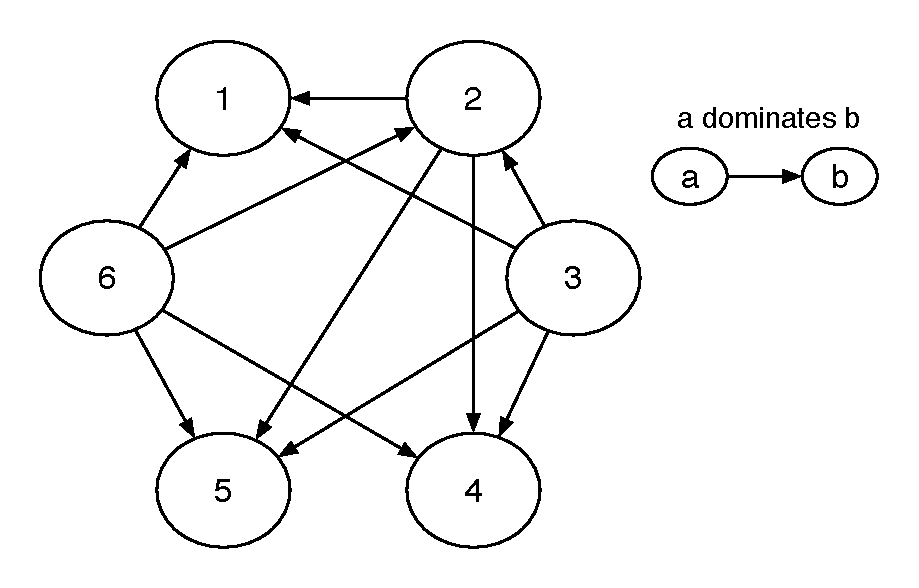
\includegraphics[scale=0.4]{pic/dominance1.eps}
			
		}{%
		\caption{Full Dominance Relationships in Graph}%
	}
	\capbtabbox
	}{%
	\caption{Full Dominance relation in Matrix Form}%
	\label{full_domin}
}
\end{floatrow}
\end{figure}







%\captionlistentry[table]{Full Dominance Relation in Matrix Form}
%\caption{Full Dominance Relation in Graphic and Matrix Forms}


In this example, applicant 2 dominates applicant 1 and applicant 3 dominates applicant 2, so the dominance between applicant 3 and applicant 1 is redundant and can be eliminated.  

\vspace{0.1in}
\textbf{Redundant Dominance Matrix:}  Graphically, a redundancy relationship from node $i$ to node $j$ states that there exists at least one two-step path (not a direct path from node $i$ to node $j$) with one intermediate node, say from node $i$ to node $k$, and then from node $k$ to node $j$ (where $k$ can be any intermediate node).  The number of two-step paths from node $i$ to node $j$ with one intermediate node can be easily calculated by 
$$ \sum_k d(i,k) \cdot  d(k,j)$$
i.e., if there exists a redundant relationship, the inner product of the two corresponding vectors should be greater or equal to 1, and 0 otherwise.  

The redundancy relationship can thus  be represented in a matrix, denoted as $D^2$,  as follows. $$D^2 = D^{f} \cdot D^{f} $$  Here $D^f$ is the original direct dominance matrix and where each entry in $D^2$ represents the number of two-step paths between a pair of applicants. 
 
\textit{Example:} Applicant 2 dominates applicant 1, and applicant 3 dominates both applicants 1 and 2, therefore the entry $d_{21}=d_{31}=d_{32}=1$. The relationship between applicant 3 and the other applicants $k$ is: $d_{3k}=(1,1,0,1,1,0)$, and applicant1 and the other applicants is $d_{k1}=(0,1,1,0,0,1) ^T $. Furthermore $\sum_k d_{3j} \cdot d_{k1}=d_{31}=1$. This represents that the relationship between applicants 1 and 3 is redundant. 


\begin{figure}
\begin{floatrow}
	\ffigbox{%
		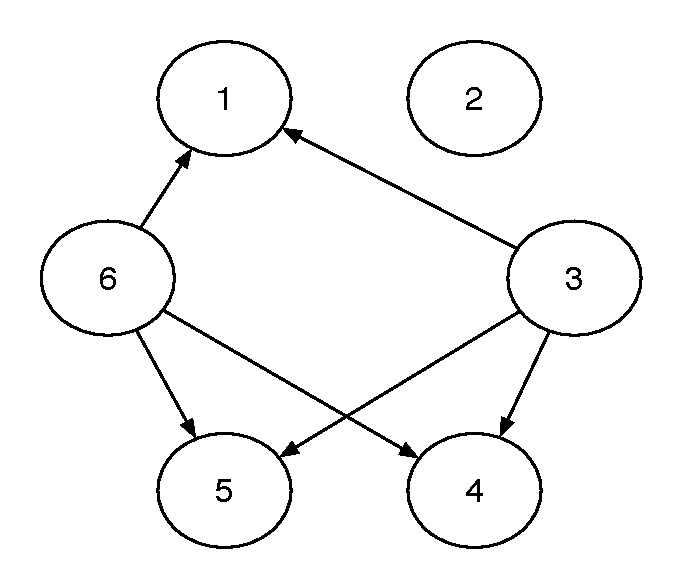
\includegraphics[scale=0.4]{pic/dominance2.eps}
		
	}{%
	\caption{Redundant Dominance Relationships in Graph}%
}
\capbtabbox
}{%
\caption{Redundant Dominance Relation in Matrix}%
\label{redundant1}
}
\end{floatrow}
\end{figure}



Finally, the elements of a \textbf{redundant matrix}, denoted as $ D_r$, can be defined as follows: 
\begin{equation}
d^{r}_{i,j} =
  \begin{cases}
  \quad  1   & \quad if d^{2}_{i,j} >= 1 \\
  \quad  0  & \quad d^{2}_{i,j} = 0 
  \end{cases}	
\end{equation}

\textbf{Minimum cardinality dominance matrix}, defined as $D_m$, can be readily defined as:
$$D_m = D_f - D_r $$
 
\textit{Example:} By eliminating redundant relationships in the graph, the minimum dominance graph and matrix forms for the example are presented Figure \ref{redundant2}:





\begin{figure}
	\begin{floatrow}
		\ffigbox{%
			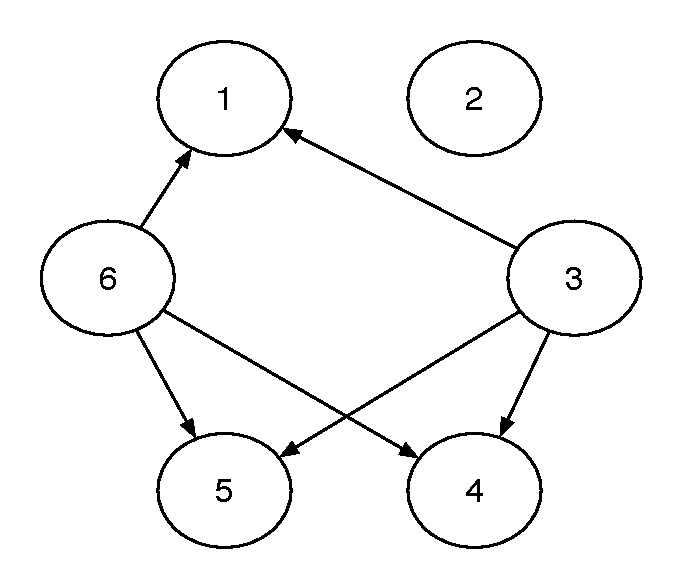
\includegraphics[scale=0.4]{pic/dominance2.eps}
			
		}{%
		\caption{Minimum Dominance in Graph}%
	}
	\capbtabbox
	}{%
	\caption{Minimum Dominance in Matrix}%
	\label{redundant2}
}
\end{floatrow}
\end{figure}


\section{Model Comparison and Results}
Computation experiment shows that the use of minimum cardinality dominance has achieved a dramatic reduction in terms of model size.  To see this, Table  \ref{model_comparison} presents the numbers of variable and constraints in respective models. Here though the number of variables has not changed, the number of constraints has been dramatically reduced, specifically the dominance constraint (\ref{constraint:2}), which composes the largest part of the model.  The original model has a total of \textbf{13,570,800} dominance constraints due to the use of direct or full dominance matrix, the reduced model, however, has only 191,497 constraints. 

% Please add the following required packages to your document preamble:
% \usepackage{multirow}
% Please add the following required packages to your document preamble:
% \usepackage{multirow}
\begin{table}[]
\centering
\begin{tabular}{|c|l|c|c|}
\hline
\multicolumn{2}{|c|}{Model Components}                                        & Original Model & Reduced Model \\ \hline
Variables                   & \multicolumn{1}{|l|}{Allocation (binary)  $x_i$} & 57,860         & 57,860        \\ \hline
\multirow{3}{*}{Constraint} & One Award per ID  (\ref{constraint:1})        & 5,260          & 5,260         \\ \cline{2-4} 
         & Dominance  (\ref{constraint:2})               & 13,570,800     & 191,497       \\ \cline{2-4} 
         & Total Budget   (\ref{constraint:3})           & 1              & 1             \\ \cline{2-4} 
         & Total Number of Constraints                   & 13,576,061     & 196,758       \\ \hline
\end{tabular}
\caption{Summary of Size of the Optimization Models }
\label{model_comparison}
\label{size_model}
\end{table}

It bears to mention that the solution of the original model with a state-of-the-art commercial solver is not possible due to memory limitations; the reduction model, however,  was solved in less than a minute on a standard laptop computer (30.15 seconds on an Apple Macbook Pro with an i7-4850HQ 2.3 GHz with 16G of RAM).

Table \ref{IPSolution}  presents the solution and the branch and bound process of the models under various budgets of 2.4M, 2.6M and 2.8M.  The university has a budget of 2.4M and the solution under that budget is used in the following analysis. 
\begin{table}[ht]
\centering
\caption{The Integer Programming Solution Process}
\label{IPSolution}
\begin{tabular}{|l|l|l|l|l|} \hline
Linear Programming & Integer Solution & Optimality Gap & Number of Nodes & Budget  \\ \hline
              19,212,184.69     & 19,212,039.66    &   0\%            &     80        &  2.4M\\ \hline
                18,899,616.21   &    18,899,275.7          &    0\%           &     0        &  2.8M \\ \hline
\end{tabular}
\end{table}

\begin{comment}

\subsubsection {Extension with Program Capacity Variations}
University have various units or programs, and typically with various capacities, that evolve over the years. Proactive marketing and optimization would help to attract as many students as possible to a business unit with capacity constraints, or minimal investment for a business unit with excess capacity (before layoffs or attrition).  The following additional notation is used in the development of capacity constraints. 
\begin{conditions*}
U & &       \quad set of business units under study, indexed by u\\
I_u & &     \quad set of students who are interested in business unit u\\
N_u & &   \quad number of resources (such as faculty members) available for unit u\\
C_u & &    \quad cost of a single resource\\
\rho_u & & \quad supervising  rate or faculty-to-student ratio for a single resource in unit u\\
Z_u & &    \quad the additional resource to be hired for each business unit u
\end{conditions*}


\begin{align}
\sum_{i \in I_u}\sum_{m \in M} x_{i,m}\cdot p^e_{i,m}\leq \rho_u\cdot N_u + \rho_u\cdot Z_u  && \forall u \in U
\end{align}

This constraint states that total number enrolled (left hand size) has to be less than the current capacity of the program, plus additional hires if necessary.  The new hires can be added to the objective function.

\end{comment}


%\chapter{Post-Processing for Financial Aid Policies}
%\todo{add model comparison}
%\todo{add regression or cluster on the results part}

\chapter{5 Policy Development \& Implementation}
The results from the optimization specifies the scholarship awards to each applicant under a specific population and budget.  The actual size and composition of application poll could be affected by the unemployment rate and is random in nature.  Nevertheless, at this stage, this study focuses on the optimization under a specific , etc. poll.  Stochastic optimization techniques such as sampling will be used to find the optimal allocation under a random enrichment and is not presented. 

\section{Derivation of Financial Aid Policies}
 The optimization result based on the above model could be sent to a general linear regression or decision tree for analysis.  Here the predictor or dependent variable is the amount of the award and the independent variables are the variables such as GPA, ACT scores, etc.  However, though it is certain variables such as Gender could affect the enrollment and graduation probabilities, thus the final allocation to applicants, awarding scholarship based on these variables are controversial; as a result, in the derivation of financial aid policies, certain variables such as gender, family  income, are not considered in the derivation of a merit-based scholarship.  

 \subsection{Financial Aid Policy Based on Decision Tree }
 The decision tree analysis is used in the derivation of the financial aid policy.  In the past two decades, decision trees, as a decision support tool,  have been commonly used in various business domains, such as direct mailing, online sales, customer retention and supplier selection, to name a few \citep{han2011data}.  

Decision tree analysis is a tree-structure model to structure  in which each internal node represents a ``test" on an attribute, each branch represents the outcome of the test and each leaf node represents a class label (decision taken after computing all attributes). The paths from root to leaf represents classification rules.  The financial aid policy from the decision tree analysis is presented in Figure \ref{FApolicybyDT}. 
 
 
 %\begin{landscape}
 \begin{figure}
  \centering
  \includegraphics[width=8in, height=5in, angle=90, origin=c]{FAPolicyDT.jpg}
 \caption{Financial Aid Policy Based on Decision Tree }
 \label{FApolicybyDT}
 \end{figure}
%\end{landscape}

% 
%todo The Policy reads as follows:  If the applicants xxxxxxxxxxxxxxxxxxxxxxx

\subsection{A Simple Financial Aid Policy Base on Stepwise Regression}
The decision tree analysis, though graphical, still seems a little complicated.  To reveal more intuitive answer to the financial aid from the optimization results, Table \ref{opt_scholar_act} presents the average financial aid with respect to the students' GPA and ACT scores. Here the row names represents the GPA scores, and the column names represent the ACT scores. The average financial aid awarded (of the optimal results with a budget of 2.8 million scholarship) is shown in the corresponding grid.  

\begin{sidewaystable}[!htbp]
 \resizebox{\linewidth}{200pt}{
\begin{tabular}{@{\extracolsep{5pt}} |l|cccccccccccccccccc|c|}
\hline
GPA/ACT  & \multicolumn{1}{c|}{18}          & \multicolumn{1}{c|}{19}          & \multicolumn{1}{c|}{20}          & \multicolumn{1}{c|}{21}          & \multicolumn{1}{c|}{22}          & \multicolumn{1}{c|}{23}   & \multicolumn{1}{c|}{24}          & \multicolumn{1}{c|}{25}          & \multicolumn{1}{c|}{26}        & \multicolumn{1}{c|}{27}         & \multicolumn{1}{c|}{28}          & \multicolumn{1}{c|}{29}          & \multicolumn{1}{c|}{30}          & \multicolumn{1}{c|}{31}         & \multicolumn{1}{c|}{32}          & \multicolumn{1}{c|}{33}          & \multicolumn{1}{c|}{34}          & 35     & Total \\ \hline
1           &                                  &                                  &                                  &                                  &     &   &                                  &                                  &     &                             &                                  &                                  &                                  &                                 &                                  &                                  &                                  &        & 0           \\ \cline{1-1} \cline{20-20} 
1.1         &                                  &                                  &                                  &                                  &                                  &                           &                                  &                                  &                                &                                 &                                  &                                  &                                  &                                 &                                  &                                  &                                  &        & 0           \\ \cline{1-1} \cline{20-20} 
1.2         &                                  & 0                                &                                  &                                  &                                  &                           &                                  &                                  &                                &                                 &                                  &                                  &                                  &                                 &                                  &                                  &                                  &        & 0           \\ \cline{1-1} \cline{20-20} 
1.3         & 0                                &                                  &                                  &                                  &                                  &                           &                                  &                                  &                                &                                 &                                  &                                  &                                  &                                 &                                  &                                  &                                  &        & 0           \\ \cline{1-1} \cline{20-20} 
1.4         &                                  & 0                                &                                  &                                  &                                  &                           &                                  &                                  &                                &                                 &                                  &                                  &                                  &                                 &                                  &                                  &                                  &        & 0           \\ \cline{1-1} \cline{20-20} 
1.5         &                                  & 0                                &                                  &                                  &                                  &                           &                                  &                                  & 0                              &                                 &                                  &                                  &                                  &                                 &                                  &                                  &                                  &        & 0           \\ \cline{1-1} \cline{20-20} 
2.5         & 0                                & 0                                & 0                                & 0                                & 0                                & 0                         & 0                                & 0                                & 0                              & 0                               & 0                                & 0                                &                                  & 0                               &                                  &                                  &                                  &        & 0           \\ \cline{1-1} \cline{20-20} 
2.6         & 0                                & 0                                & 0                                & 0                                & 0                                & 0                         & 0                                & 0                                & 0                              & 0                               &                                  & 1250                             & 1500                             &                                 &                                  & 1500                             &                                  &        & 25.8 \\ \cline{1-1} \cline{20-20} 
2.7         & 0                                & 0                                & 0                                & 0                                & 0                                & 0                         & 0                                & 0                                & 0                              & 0                               & 1500                             &                                  & 2000                             &                                 &                                  &                                  &                                  &        & 24.2 \\ \cline{1-1} \cline{20-20} 
2.8         & 0                                & 0                                & 0                                & 0                                & 0                                & 0                         & 0                                & 0                                & 0                              & 300                             & 1500                             & 2000                             &                                  &                                 &                                  & 2500                             &                                  &        & 39.4 \\ \cline{1-1} \cline{20-20} 
2.9         & 0.0                              & 0.0                              & 0.0                              & 0.0                              & 0.0                              & 0.0                       & 0.0                              & 0.0                              & 818.2                          & 1875.0                          & 2000.0                           &                                  &                                  &                                 &                                  &                                  &                                  &        & 63.4        \\ \cline{1-1} \cline{20-20} 
3           & 0.0                              & 0.0                              & 0.0                              & 0.0                              & 0.0                              & 0.0                       & 0.0                              & 1166.7                           & 1500.0                         & 2000.0                          & 2000.0                           & 2200.0                           &                                  & 3200.0                          &                                  &                                  & 5200.0                           &        & 216.3       \\ \cline{1-1} \cline{20-20} 
3.1         & 0.0                              & 0.0                              & 0.0                              & 0.0                              & 0.0                              & 0.0                       & 523.8                            & 1500.0                           & 1727.3                         & 2000.0                          & 2000.0                           & 2500.0                           & 2500.0                           &                                 &                                  &                                  &                                  & 7300.0 & 276.7       \\ \cline{1-1} \cline{20-20} 
3.2         & 0.0                              & 0.0                              & 0.0                              & 0.0                              & 0.0                              & 781.3                     & 1000.0                           & 1750.0                           & 2000.0                         & 2250.0                          & 2500.0                           & 2500.0                           & 2780.0                           & 3950.0                          & 5200.0                           &                                  &                                  &        & 573.7       \\ \cline{1-1} \cline{20-20} 
3.3         & 0.0                              & 0.0                              & 0.0                              & 0.0                              & 647.1                            & 1000.0                    & 1613.6                           & 2000.0                           & 2315.8                         & 2500.0                          & 2920.0                           & 3200.0                           & 3866.7                           & 4200.0                          &                                  & 5200.0                           & 5200.0                           &        & 962.8       \\ \cline{1-1} \cline{20-20} 
3.4         & 0.0                              & 0.0                              & 0.0                              & 694.4                            & 1000.0                           & 1550.0                    & 2000.0                           & 2000.0                           & 2500.0                         & 2990.0                          & 3200.0                           & 3200.0                           & 4200.0                           & 4200.0                          &                                  &                                  &                                  &        & 1185.1      \\ \cline{1-1} \cline{20-20} 
3.5         & 0.0                              & 0.0                              & 695.7                            & 1000.0                           & 1724.1                           & 2000.0                    & 2000.0                           & 2216.7                           & 2500.0                         & 3200.0                          & 3200.0                           & 3200.0                           & 4200.0                           & 4200.0                          &                                  & 5200.0                           &                                  &        & 1696.7      \\ \cline{1-1} \cline{20-20} 
3.6         & 0.0                              & 545.5                            & 1000.0                           & 1000.0                           & 2000.0                           & 2000.0                    & 2357.1                           & 2500.0                           & 2864.0                         & 3200.0                          & 3200.0                           & 3800.0                           & 4200.0                           & 4200.0                          & 5200.0                           & 5200.0                           & 5200.0                           &        & 2148.1      \\ \cline{1-1} \cline{20-20} 
3.7         & 0.0                              & 1000.0                           & 1000.0                           & 1500.0                           & 2000.0                           & 2285.7                    & 2500.0                           & 2945.5                           & 3200.0                         & 3200.0                          & 3700.0                           & 4200.0                           & 4200.0                           & 5200.0                          & 5200.0                           &                                  & 5200.0                           &        & 2532.8      \\ \cline{1-1} \cline{20-20} 
3.8         & 0.0                              & 1000.0                           & 1000.0                           & 2000.0                           & 2000.0                           & 2500.0                    & 3006.9                           & 3200.0                           & 3200.0                         & 4014.8                          & 4200.0                           & 4200.0                           & 4900.0                           & 5200.0                          & 5200.0                           & 5200.0                           &                                  &        & 3007.5      \\ \cline{1-1} \cline{20-20} 
3.9         & 666.7                            & 1000.0                           & 1000.0                           & 2000.0                           & 2000.0                           & 2500.0                    & 3200.0                           & 3200.0                           & 3680.0                         & 4200.0                          & 4200.0                           & 4644.4                           & 5200.0                           & 5200.0                          & 5200.0                           & 5200.0                           & 5200.0                           &        & 3360.4      \\ \cline{1-1} \cline{20-20} 
4           &                                  & 1000.0                           & 1000.0                           & 2000.0                           & 2000.0                           & 2500.0                    & 3200.0                           & 3200.0                           & 4200.0                         & 4808.7                          & 5200.0                           & 5200.0                           & 5200.0                           & 5200.0                          & 5200.0                           & 5200.0                           & 6542.9                           & 7300.0 & 4186.1      \\ \cline{1-1} \cline{20-20} 
4.1         &                                  & 1000.0                           & 1000.0                           & 2000.0                           & 2000.0                           & 2500.0                    & 3200.0                           & 3200.0                           & 4200.0                         & 5200.0                          & 5200.0                           & 5200.0                           & 5200.0                           & 5200.0                          & 5200.0                           & 5200.0                           & 7300.0                           &        & 3982.1      \\ \cline{1-1} \cline{20-20} 
4.2         & 1000.0                           &                                  & 1000.0                           & 2000.0                           & 2000.0                           & 2500.0                    & 3200.0                           & 3200.0                           & 4200.0                         & 5200.0                          & 5200.0                           & 5200.0                           & 5200.0                           & 5200.0                          & 5200.0                           & 5200.0                           & 7300.0                           &        & 4175.0      \\ \cline{1-1} 
4.3         &                                  &                                  &                                  &                                  & 2000.0                           & 2500.0                    & 3200.0                           & 3200.0                           & 4200.0                         & 5200.0                          & 5200.0                           & 5200.0                           & 5200.0                           & 5200.0                          & 5200.0                           & 5200.0                           & 7300.0                           &        & 4607.9      \\ \cline{1-1} \cline{20-20} 
4.4         &                                  &                                  &                                  &                                  &                                  &                           & 3200.0                           & 4200.0                           & 5200.0                         & 5200.0                          & 5200.0                           & 5200.0                           & 5200.0                           & 5200.0                          & 5200.0                           & 5200.0                           & 7300.0                           &        & 5125.0      \\ \cline{1-1} \cline{20-20} 
4.5         &                                  &                                  & 1000.0                           &                                  & 2000.0                           & 2925.0                    &                                  & 5200.0                           & 5200.0                         &                                 & 5200.0                           & 5200.0                           &                                  & 5200.0                          & 5200.0                           & 6233.3                           &                                  & 7300.0 & 4605.3      \\ \cline{1-1} \cline{20-20} 
4.6         &                                  &                                  &                                  &                                  &                                  & 4200.0                    &                                  &                                  & 5200.0                         & 5200.0                          & 5200.0                           &                                  & 5200.0                           &                                 & 5900.0                           & 7300.0                           & 7300.0                           &        & 5730.0      \\ \cline{1-1} \cline{20-20} 
4.7         &                                  &                                  &                                  & 5200.0                           &                                  &                           &                                  &                                  & 5200.0                         & 5200.0                          & 6200.0                           &                                  &                                  & 8400.0                          & 8400.0                           & 8400.0                           &                                  &        & 6377.8      \\ \cline{1-1} \cline{20-20} 
4.8         &                                  &                                  &                                  &                                  &                                  &                           &                                  &                                  &                                & 5200.0                          & 6200.0                           &                                  & 6200.0                           &                                 &                                  &                                  &                                  &        & 5866.7      \\ \hline
Grand Total & \multicolumn{1}{c|}{7.2} & \multicolumn{1}{c|}{92.7} & \multicolumn{1}{c|}{166.2} & \multicolumn{1}{c|}{428.7} & \multicolumn{1}{c|}{787.1} & \multicolumn{1}{c|}{1206} & \multicolumn{1}{c|}{1664.8} & \multicolumn{1}{c|}{2112} & \multicolumn{1}{c|}{2642.1} & \multicolumn{1}{c|}{3407.5} & \multicolumn{1}{c|}{3835.6} & \multicolumn{1}{c|}{3981.3} & \multicolumn{1}{c|}{4561.4} & \multicolumn{1}{c|}{4784.9} & \multicolumn{1}{c|}{5323.2} & \multicolumn{1}{c|}{5258.8} & \multicolumn{1}{c|}{6247.6} & 7300   & 1134.7 \\ \hline
\end{tabular}}
\caption{Optimization Mean Scholarship vs GPA and ACT}
\label{opt_scholar_act}
\end{sidewaystable}

These results clearly suggest a strong relationship between the awards and both GPA and ACT scores.  As a result, a \textit{composite score} index, calculated as $10 \times GPA + ACT $ was proposed by the enrollment team to capture the applicants academic merits and used as the basis of the award.

Figure \ref{compositescore} presents the average award from the optimization results for the composite score. Here, the horizontal axis represents the composite score and the vertical axis the average scholarship awarded for the corresponding score. 
 \begin{figure}[ht]
   \centering
 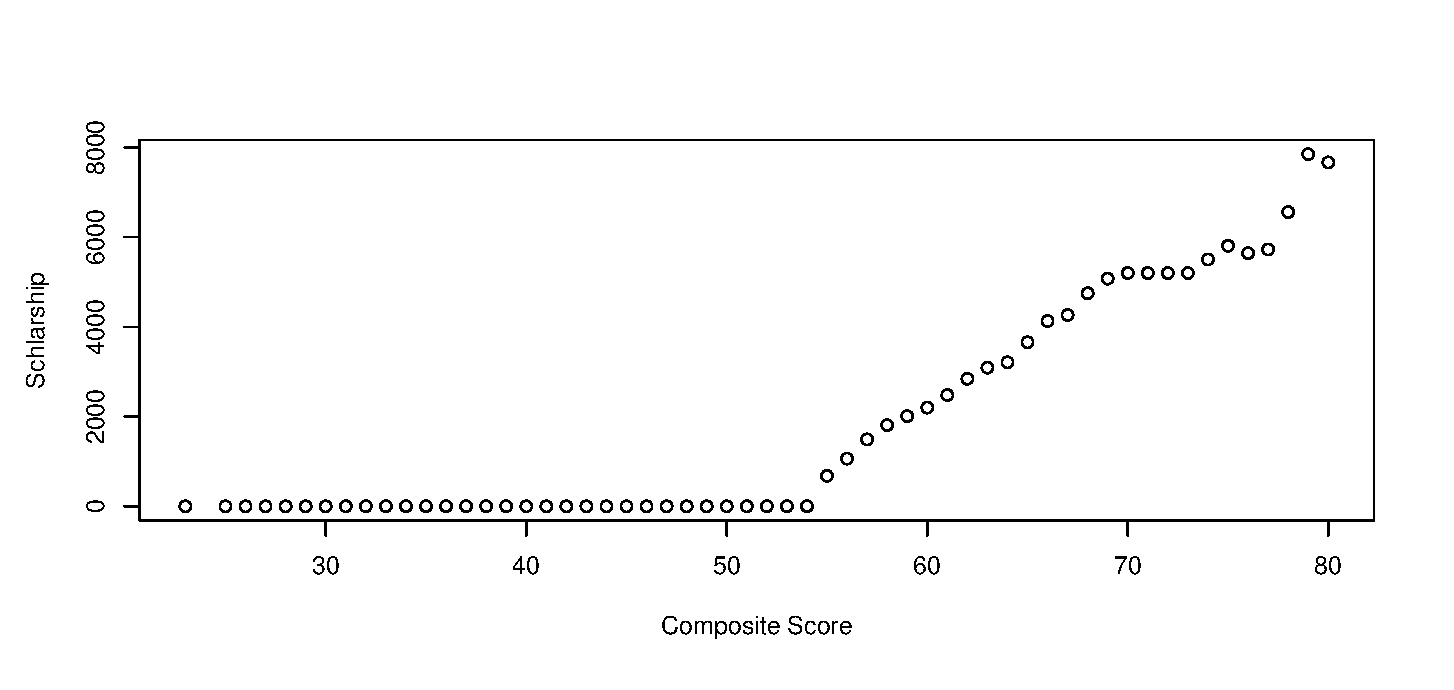
\includegraphics[scale=0.65]{pic/scho_composite.eps}
 \caption{Scholarship versus composite score}
 \label{compositescore}
\end{figure}

The figure clearly shows that no scholarship should be awarded when the combined score is below 54.  A linear relationship seems to exist between the scholarship and the composite score when the composite score is between 55 and 70, and the scholarship seems to remain the same when the score is above 70. Use ``CS'' as the variable representing the composite score, a piecewise regression is used to capture these observations and the resulting regression equations are shown in Table \ref{money_result} and a graph of the piecewise regression is shown in \ref{AppB}. A simpler discretized version of the scholarship policy is shown in Table \ref{money_result_discrete}.

\begin{table}[ht]
\centering
\begin{tabular}{|c|c|c|}
\hline
Composite Score & \# of Applicants & Scholarship Amount \\ \hline
0-53.9         & 2,897	&0              \\ \hline
54-68.9        & 2,103  &$309\times CS -16,380 $            \\ \hline
69-76.9        &  241 &  $101\times CS - 2,024$           \\ \hline
77-80       & 19 &   $711 \times CS -48,910$          \\ \hline
\end{tabular}
\caption{Piecewise Scholarship Allocation}
\label{money_result}
\end{table}


\begin{table}[ht]
\centering
\begin{tabular}{|c|c|}
\hline
Composite Score & Scholarship Amount \\ \hline
0-54.9         & 0              \\ \hline
55-59.9         & 1,500              \\ \hline
60-65.9         & 2,500              \\ \hline
66-69.9         & 3,500              \\ \hline
70-74.9         & 4,500              \\ \hline
75+             & 6,000              \\ \hline
\end{tabular}
\caption{Discretized Version of Scholarship Allocation}
\label{money_result_discrete}

\end{table}

\begin{comment}
\subsection{Comparison of Policies} 

Feeding Back these policies into the optimization model, table \ref{policy_compare} presents the results of various policies. Here  the Objective column represents the objective values, Enrollment represents the expected enrollment; the graduation represents the expected number of graduation; tuition represents the expected tuition income, and SSI represents the expected SSI from state when applicant enroll and graduate.



	
\begin{table}[]
\centering
\caption{My caption}
\label{my-label}
\begin{tabular}{|l|l|l|l|l|l|} \hline
Policy                        & Objective & Enrollment & Graduation& Tuition & SSI  \\ \hline \hline
Optimization Result &                 &                   &                   &                  &                     \\ \hline
Decision Tree Model  &                 &                   &                   &                  &                     \\ \hline
Stepwise Regression Model     &                 &                   &                   &                  &                     \\ \hline
Discrete Stepwise Regression  &                 &                   &                   &                  &                     \\ \hline
Current Policy                &                 &                   &                   &                  &                    \\ \hline
\end{tabular}
\label{policy_compare}
\end{table}

As can be seen, it s expected that a 10\% increase in enrollment from *** to ** if we adopted the optimal result and perform individualize scholarship.  DT tree analysis and stepwise regression and discrete stepwise regression based on composite scores ********  

Out of the composite scores, DT preforms best , followed by Stepwise 
\end{comment}


\section{Implementation and Results}
The scholarship allocation based on the composite score and the policy presented in Table \ref{money_result} has been used as the foundation for the scholarship for the university in the 2013 to 2014 academic year.  A proactive approach has been taken by the university. The enrollment and admission office has purchased data on student performance and  scholarship awards before they even apply (these awards hinge upon the verification of their official performance). For details, please see \url{http://www.wright.edu/raider-connect/financial-aid/first-year-scholarships}.


Table \ref{enroll_stats} presents the enrollment statistics for the university in the 2012 - 2013 academic year and those of the 2013 - 2014 academic year. 

\begin{table}[ht!]
\centering
\begin{tabular}{|c|c|c|c|c|}
\hline
                               & 2013 & 2014 & \# Increase & \% Increase \\ \hline
Application                    & 6,101 & 6,068 & -43         & -0.7\%      \\ \hline
Admitted                       & 4,541 & 4,773 & 232         & 5.1\%       \\ \hline
Non-Scholarship                & 2,166 & 2,157 & -9          & -0.4\%      \\ \hline
Scholarship Award              & 2,375 & 2,616 & 241         & 10.1\%      \\ \hline
%\% of scholarship              & 52\% & 55\% &             &             \\ \hline
Matriculated                   & 2,001 & 2,222 & 221         & 11.0\%      \\ \hline
%Non-Scholarship Student        & 931  & 1000 & 69          & 7.4\%       \\ \hline
%Scholarship Student            & 1070 & 1222 & 152         & 14.2\%      \\ \hlineloc
%Scholarship Matriculation Rate & 45\% & 47\% &             &             \\ \hline
\end{tabular}
\caption{Enrollment Statistics for the 2012-2013 and 2013-2014 Academic Years}
\label{enroll_stats}

\end{table}

In 2012-2013, there are a total of 6,101 applicants, of them,4,541   are admitted. 2,375 were awarded scholarships and 2,166 were not scholarships. 52\% of the students were awarded scholarships, and a total of 2,001 students matriculated. 

In the 2013-2014 academic year, there were a total of 6,068 applicants; of them, 4,773 were admitted, 2,616 were awarded scholarships and 2,157 were not awarded scholarships, 56\% of the students are awarded scholarships and a total of 2,222 students matriculated. 

Notice that the number of applicants does not change dramatically, actually showing a reduction of -43 (-0.7\% increase), but the actual enrollment increased by 221  or 11.0\% over the previous years.  It is believed that the use of the optimal policy could generate millions of dollars or in revenue for the university in the next few years. 

\section{Time Line}

Several tasks need to be completed in the remaining year and the intended graduation and thesis defense is August 2017.  These tasks and time lines are presented in Table \ref{timeline}. 

\begin{table}[ht]
\centering

\begin{tabular}{|l|l|}
\hline
Tasks                                                                & Time Line \\ \hline
Development and Comparison of Other Prediction Methods               &  9/2016               \\ \hline
Optimization Result Comparison of Various Budget Constraints          & 10/2016               \\ \hline
Optimization Result Under Different Applications Pool			 &       11/2016          \\ \hline
Finish Writing Papers and Submit Thesis                             		&  2/2017               \\ \hline
\end{tabular}
\caption{Future Study}
    \label{timeline}
\end{table}


\begin{comment}
\section{Implementation}


In an attempt to improve the academic profile of our new, direct from high school class of all 2013 and to address capacity for growth within the colleges, the  financial aid office did a study: WSU awarded additional scholarship funds to students who were direct admits into some colleges. The students targeted had an average HS GPA of 3.97 and an ACT of 27+. Overall this funding proved to be very successful because the number of students who enrolled with a HS GPA of 4.0 and greater increased by 51\% and the students who had an ACT of 31+ increased by 18\%. WSU matriculated an additional 34\% of students in this group due to the additional funding.
 %This effort began our scholarship leveraging efforts, and we had good results considering the timing of the original project. 
    	
After an extensive data review process, we found that because the average award for this group of students increased to \$3,500-\$4,500 (full in-state tuition is \$8,354), WSU were able to attract higher achieving students with the additional scholarships, by meeting their `need'\ for competitive merit-based scholarships. WSU were competitive with our peers by percentage of tuition discounted for this group.

We initiated the study in the 2013 Fall semester to redesign our merit-based scholarship structure aiming to increase the headcount without sacrificing academic profile. At the same time, a massive marketing campaign lead by the school administration kicked off. Since more than 95\% of the incoming students at WSU are Ohio residents, our study is focus on this group of students. 

Application data from 2006 to 2013 was collected via the enrollment office. The data contains mainly two categories: students academic profiles and economic status. More details are included in the study approach portion of this study.
\end{comment}

% Study on enrollment management falls into two main areas \citet{maltzdecision}: developing predicting models for enrollment levels and on systems for identifying expected targeting applicants. And the prediction models largely consist of two levels \citet{aksenovaenrollment}: (1) curve-fitting techniques such as moving averages, exponential smoothing, spectral analysis; (2) data mining models such as regression models, tree structure models, stochastic models.

%\chapter{Sensitivity Analysis and Insights}

\appendix
\chapter{Appendix A: Summary Statistics of Data Fields Provided by the University}  \label{app A}

%\section{Variables used in the model}

%The variable used in the model contains both continuous and discrete variables and are listed in the table below. 

\begin{table}[ht]
\centering
\caption{Description of Data Fields (Variables)}
\label{my-label}
\begin{tabular}{ll}
\hline
Variable Name     & \multicolumn{1}{c}{Description}      \\ \hline
MATRICULATION     & Whether applicant enrolled or not           	  \\
GPA               & High school GPA                                   \\
ACT               & ACT score                       					\\
HS.PERCENTILE     & Applicant's high school percentile         \\
GENDER            & Male or female                       \\
ETHNICITY         & Ethnicities                               \\
UNDERREPRESENTED  & 1 if the applicant is white; 0 otherwise       \\
%HS.RAIDER.COUNTRY & Whether high school graduate tend to go to WSU\\
HS.DESC           & Applicant's high school                       \\
TUITION           & Tuition of the school year                          \\
PELL.GRANT        & Applicant's Pell grant information       \\
SCHOLARSHIP       & How much scholarship the applicant got     \\
TOTAL.FREE.MONEY  & SCHOLARSHIP+PELL.GRANT                         \\
OUT.OF.POCKET     & TUITION-Total.FREE.MONEY              \\
APP.COLLEGE       & Intended college            \\
APP.MAJOR         & Intended major                \\ \hline
\end{tabular}
\end{table}
	
% Table created by stargazer v.5.2 by Marek Hlavac, Harvard University. E-mail: hlavac at fas.harvard.edu
% Date and time: Sun, Feb 21, 2016 - 17:20:56
\begin{table}[ht] \centering 
  \caption{Summary Statistics, mean, standard deviation, median, mim, and max, of Selected Continuous Variables} 
  \label{Continuous} 
\begin{tabular}{@{\extracolsep{5pt}} cccccccccccccc} 
\\[-1.8ex]\hline 
\hline \\[-1.8ex] 
  & mean & sd & median  & min & max  \\
\hline \\[-1.8ex] 
GPA   &$3.0$ & $0.6$ & $3.1$  & $0.4$ & $4.9$  \\ 
ACT   & $21.2$ & $4.3$ & $21$ & $8$ & $36$    \\ 
PELL.GRANT  & $1,452$ & $2,228$ & $0$ & $0$ & $5,550$  \\ 
OUT.OF.POCKET  & $5,455$ & $2,467$ & $6,278$  & $$-$5,935$ & $8,354$   \\ 
DISTANCE.NUM &  $57.6$ & $53.4$ & $43.8$  & $2.6$ & $276.7$   \\ 
\hline \\[-1.8ex] 
\end{tabular} 
\end{table}

\begin{table}[ht]
\centering
\caption{Summary of Enrollment and Not Enrollment of Various Regions (Tier 1: Tire 2: Tire 3: .....s) }
\label{tier}
\begin{tabular}{|c|c|c|}
\hline
HS.Tier & Enrolled & Not Enrolled \\ \hline
Tier 1  & 8013     & 5500         \\ \hline
Tier 2  & 2524     & 2570         \\ \hline
Tier 3  & 661      & 623          \\ \hline
Tier 4  & 2470     & 4123         \\ \hline
Tier 5  & 1296     & 2469         \\ \hline
Tier 6  & 2228     & 2866         \\ \hline
\end{tabular}
\end{table}

\begin{table}[ht]
\centering
\caption{Summary of Enrollment and Not Enrollment by Ethnicity}
\label{ethnicity}
\begin{tabular}{|c|c|c|}
\hline
Ethnicity             & Enrolled & Not Enrolled \\ \hline
Asian                 & 350      & 347          \\ \hline
African American      & 3,332     & 3,984         \\ \hline
Hawaiian              & 19       & 11           \\ \hline
Hispanic              & 403      & 413          \\ \hline
Native Indian/Alaskan & 40       & 35           \\ \hline
Two/More              & 583      & 375          \\ \hline
Unknown               & 156      & 418          \\ \hline
White                 & 12,309    & 12,568        \\ \hline
\end{tabular}
\end{table}

\begin{table}[h]
\centering
\caption{Summary of Enrollment and Not Enrollment by College}
\label{college}
\begin{tabular}{|c|c|c|}
\hline
College                    & Enrolled & Not Enrolled \\ \hline
College of Business        & 1825     & 1984         \\ \hline
College of Science \& Math & 2573     & 2688         \\ \hline
College of Liberal Arts    & 3086     & 3604         \\ \hline
College of Education       & 1609     & 1784         \\ \hline
College of Engineering     & 2331     & 2097         \\ \hline
College of Nursing         & 2338     & 2373         \\ \hline
University College         & 3430     & 3621         \\ \hline
\end{tabular}
\end{table}

\begin{table}[h]
\centering
\begin{tabular}{|c|c|c|}
\hline
Gender & Enrolled & Not Enrolled \\ \hline
Female  & 9,922     & 10,784        \\ \hline
Male   & 7,270     & 7,367         \\ \hline
\end{tabular}
\caption{Summary of Enrollment by Gender}
\label{enroll_gender}
\end{table}


\begin{figure}[ht]
   \centering
 \includegraphics[scale=0.65]{pic/applicant_unmployment.eps}
 \caption{Applicants vs Unemployment Rate}
\end{figure}


\chapter{Appendix B: Piecewise Regression for Scholarship}  \label{AppB}

\begin{figure}[ht]
   \centering
 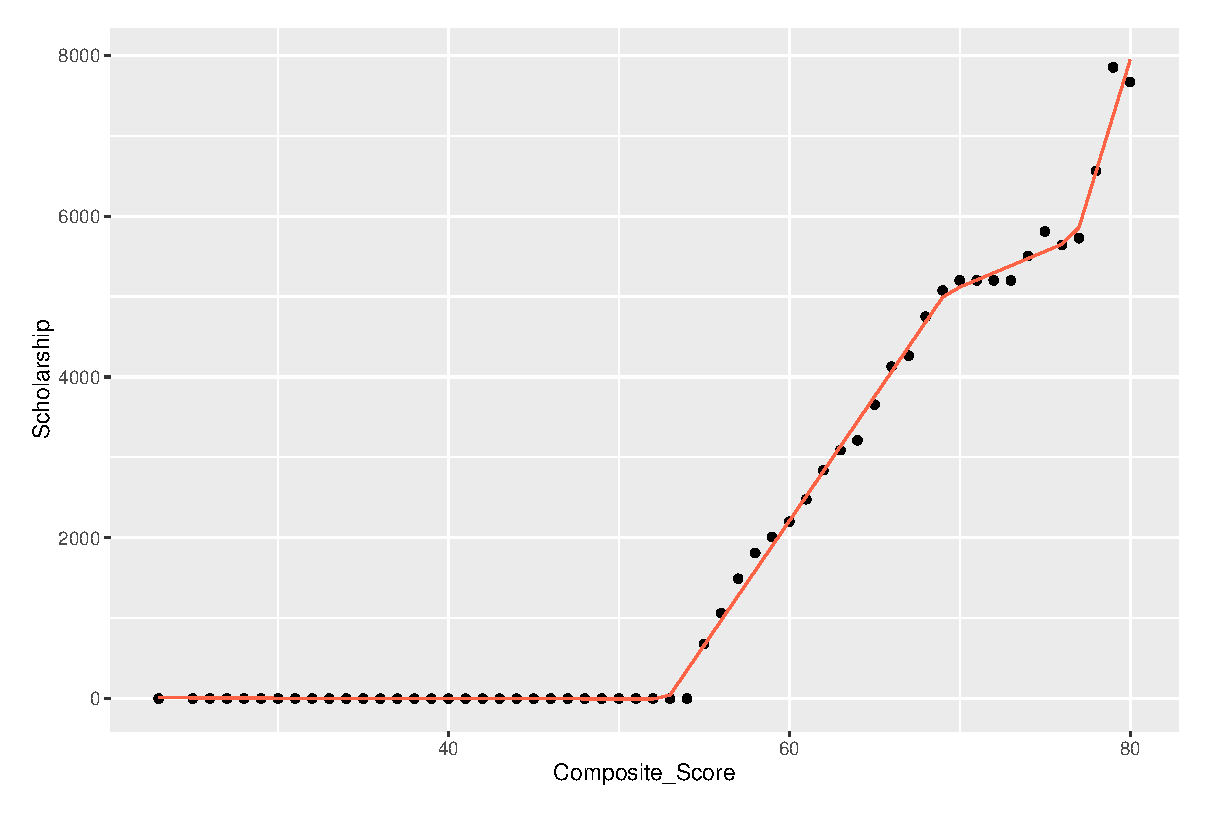
\includegraphics[scale=0.75]{pic/PieceWiseRegression.eps}
 \caption{PieceWise Linear Regression Result and the Original Results}
 \label{PieceWisePolicy}
\end{figure}




\begin{comment}
The response variables in the enrollment and graduation models are:
\begin{itemize}
	\item MATRICULATION. Whether the applicant enrolled or not.
	\item DEGREE.AWARDED. Whether the enrolled applicant graduated or not.
\end{itemize}

The variables represent applicant's academic performance in the model include: 
\begin{itemize}
	\item GPA. The high school GPA of the applicant. The range of the GPA is 0.5 to 5. Some high school students take AP or college classes so that the GPA is larger than 4.0.
	\item  ACT. The highest ACT composite score that applicant reported. Applicant only submit the highest ACT composite score. For student who took SAT, the score was converted to ACT according to \citep{ACTSAT}.
	\item HS.Percentile, ranging from 1 to 100, the applicant's percentile from the high school, which is an easy way to represent applicant's standing at graduation relative to other graduate.
\end{itemize}

The variables related to applicant's financial status include:
\begin{itemize}
	\item TUITION. The amount of tuition that a applicant pays before the deduction of any types of aids. Since this study does not include the out-of-state applicants, the tuition are equal for all the applicants.
	\item Family Effective Contribution (EFC). This variable is used to get the Pell Grant information.
	\item Pell Grant. The Pell Grant is converted from EFC, which followed by the metric got from \citep{EFC_Pell}. There are 8560 applicants who did not fill the EFC information in the data. I assumed these applicants knew that they did qualify any Pell Grant, so that the NAs were converted to the lowest EFC which does not qualify any Pell Grant.
	\item SCHOLARSHIP. The amount amount of money applicant promised in the enrollment stage.
	\item TOTAL.FREE.MONEY. This variable is calculated as SCHOLARSHIP + PELL GRANT. It represents that all the aids that one applicant got.
	\item OUT.OF.POCKET. It is calculated as TUITION - Total.FREE.MONEY. This indicates how much money does one applicant needs to pay.
	\item UNEMPLOYMENT.INDEX. The school year Ohio unemployment rate was added to reflect the overall economy. It is known that college is the safe harbor when economy underperforms \citep{barr2015out}.
\end{itemize}

The personal information variables include:
\begin{itemize}
	\item GENDER. Applicant's gender.
	\item HS.COUNTY.TIER. Since Wright State University is a commuter school, the distance between home and campus could be an important factor. This variable relates to the distance from the county in which the applicant lived, to Wright State. There were six tiers in all, as well as “Out of State/Unknown” subcategory. Tier 1 included students who lived in: Clark, Greene, Miami and Montgomery counties. Tier 2: Butler, Champaign, Clinton, Darke, Preble and Warren counties. Tier 3: included Auglaize, Mercer and Shelby counties. Tier 4 included Franklin, and Hamilton counties. Tier 5 was northern Ohio counties. And Tier 6 was all other Ohio counties. As you can see, Tier 1 includes the counties closest to Wright State, and Tier 5, 6/Out of State include the counties furthest from Wright State.
	\item HS.DISTANCE. The numeric value of distance between high school and campus are also added.

	\item ETHNICITY. This variable has several different ethnicities: BlackOrAfricanAmerican, White, Asian, Hispanic, TwoMore.
	\item APP.COLLEGE. The intended college of a applicant.
\end{itemize}

\end{comment}

%-----------------------------------------------------------------------
% Bibliography
%-----------------------------------------------------------------------
\clearpage \phantomsection %used to correctly anchor hyperlinks
\renewcommand\baselinestretch{1.5}
%\addcontentsline{toc}{chapter}{Bibliography}
%\bibliographystyle{apalike}
\bibliographystyle{plainnat}
\bibliography{shuai_cita}


\renewcommand\baselinestretch{1.25}

\end{document} 	

